\documentclass{article}
\usepackage[utf8]{inputenc} % Codificación de entrada UTF-8
\usepackage{graphicx} 
\usepackage{fancyhdr}
\usepackage{ragged2e}
\usepackage{multirow}
\usepackage[hidelinks]{hyperref}
\usepackage[table,xcdraw]{xcolor}
\usepackage{ulem}
\usepackage{listings}
\usepackage[spanish]{babel} % Paquete para idioma español
\usepackage{xcolor} % Para usar colores

\usepackage{bbding}
\usepackage{pifont}
\usepackage{wasysym}
\usepackage{amssymb}

\definecolor{verdeCompletado}{RGB}{0, 128, 0} % Verde para tareas completadas
\definecolor{azulProgreso}{RGB}{30, 144, 255} % Azul para tareas en progreso
\definecolor{grisPendiente}{RGB}{169, 169, 169} % Gris para tareas pendientes

\usepackage{pgfgantt}
\usepackage{float}
\usepackage{pdflscape} % Paquete para la orientaci\'on horizontal
\usepackage{longtable} % Para tablas largas.
\usepackage{geometry} 
\usepackage{translator}
\ganttset{calendar week text={\small{\startday/\startmonth}}}

\newcommand\textganttbar[5][]{%
    \ganttbar[#1,bar/.append style={alias=tmp}]{#2}{#4}{#5}
    \path 
    let
    \p1=(tmp.west),\p2=(tmp.east),
    \n1={\x2-\x1},\n2={width("#3")},
    \n3={ifthenelse(\n1>\n2,90,270)}
    in
    node [anchor=\n3,font=\footnotesize] at (tmp.north) {#3};
}

% Definir un color azul oscuro
\definecolor{azulOscuro}{RGB}{0, 0, 139} % Azul oscuro

% Adicionales
\addto\captionsspanish{\renewcommand{\contentsname}{\'Indice}} % Cambio de Contents a \'Indice

\pagestyle{fancy}
\fancyhf{}
\lhead{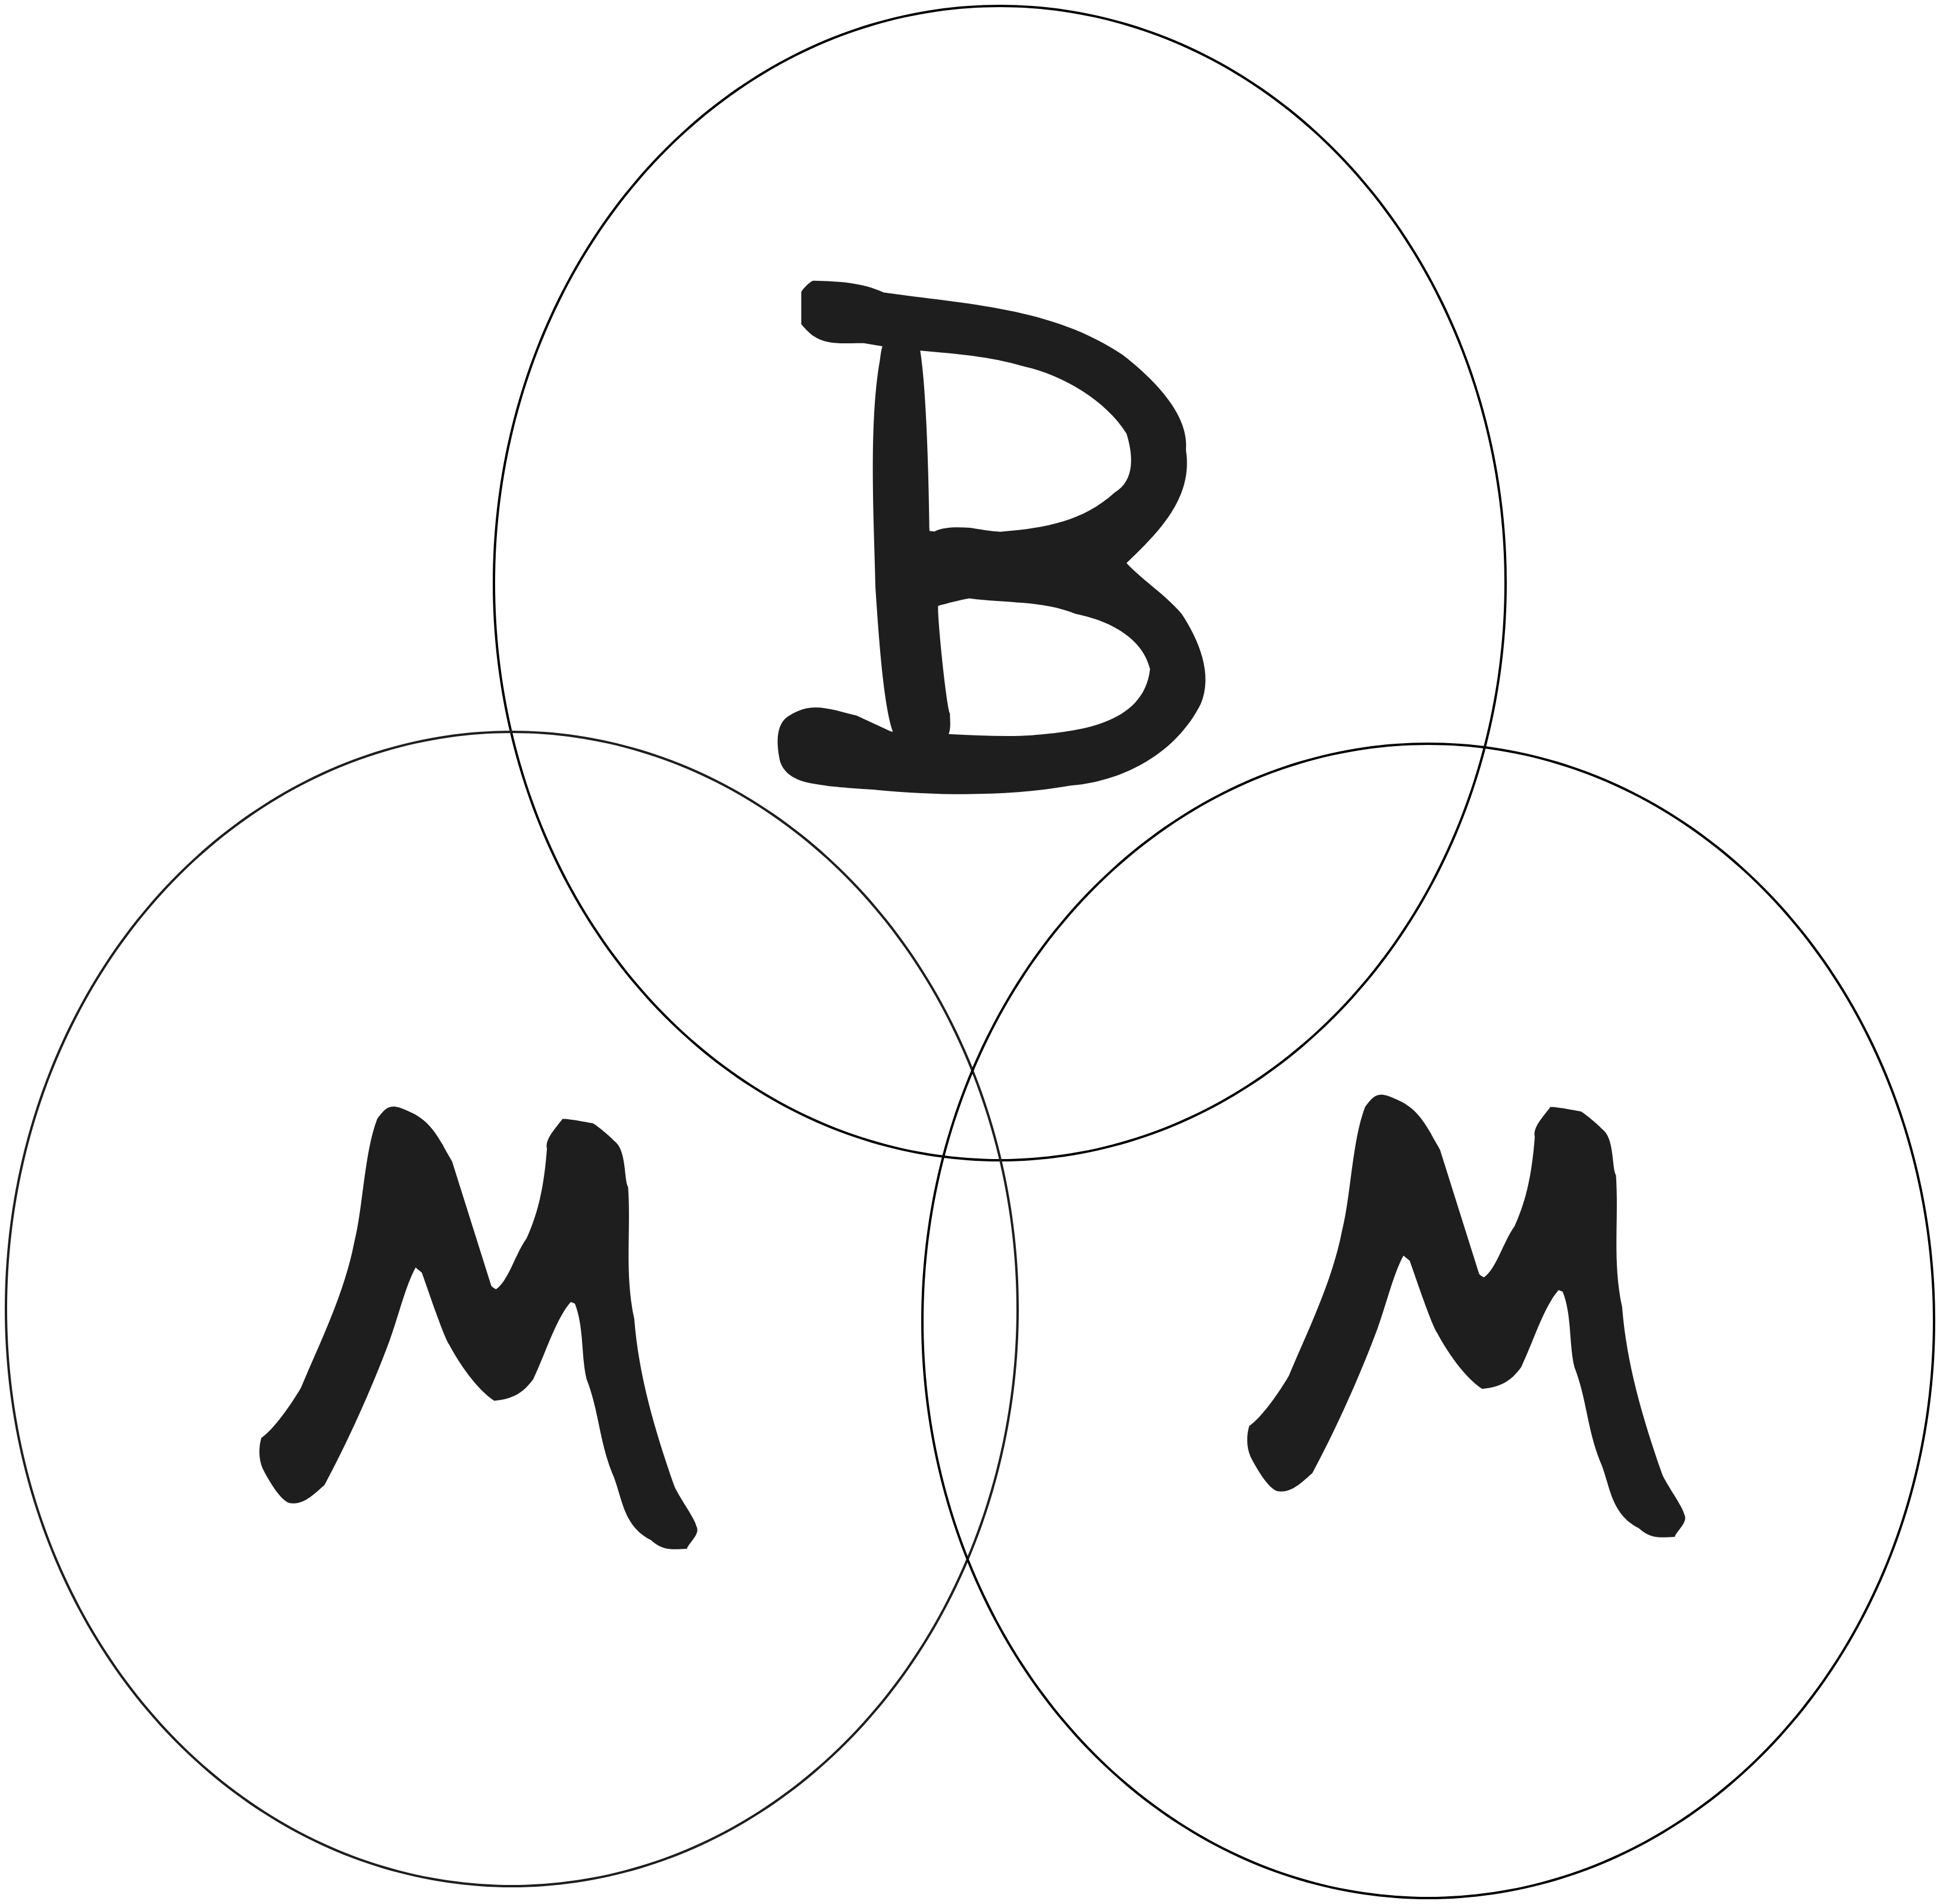
\includegraphics[width=1cm]{TFG/Logo.png}}
\rhead{
\includegraphics[width=1cm]{TFG/fotomain.png}} 

\renewcommand{\headrulewidth}{3pt}

% Comienzo de Documento
\begin{document}
    % Creaci\'on de Portada
   \begin{titlepage}
        \begin{center}
            {\scshape\large{Grado Superior}}\\
            {\scshape\large{Desarrollo de aplicaciones multiplataforma}} \\

            \vspace{2cm}
            {
\includegraphics[width=0.4\textwidth]{TFG/fotomain.png}} \par
            \vspace{2cm}
            {\scshape\large{Aplicaci\'on para la Gesti\'on de Tareas y Control \\ de Alimentos en el Hogar}\\
            \vspace{2cm}
            \textbf{TaskTracer}}} \\
            \vspace{2cm}
            {\Large Autor:} \\
            \vspace{1mm}
            {\Large Borja Merch\'an Mckenna} \\
            \vspace{1mm}
            {\Large 26/11/2024}
        \end{center}
    \end{titlepage}

    % Comienzo de \'Indice
    \clearpage
    \tableofcontents   % \'Indice de contenido
    \listoffigures      % Lista de figuras

    % Secci\'on de Introducci\'on
    \clearpage
    \begin{flushleft}
    \justifying

\section{Metodolog\'ia, Leyes y Normativas}
\subsection{Metodolog\'ia Realizada del Proyecto}
Para llevar a cabo el proyecto, se ha empleado una combinaci\'on de diferentes t\'ecnicas y herramientas adecuadas a las tareas que lo exig\'ian. Se ha utilizado un enfoque iterativo e incremental, lo que permiti\'o adaptarse a los cambios que surgieron a lo largo del desarrollo. Adem\'as, se implement\'o una metodolog\'ia basada en el uso del diagrama de Gantt, lo cual facilit\'o la planificaci\'on y organizaci\'on de las tareas de manera flexible.

\subsection{Leyes y Normativas}
Dado que el proyecto incluye funcionalidades relacionadas con la gesti\'on de usuarios y datos, es fundamental garantizar el cumplimiento de las normativas vigentes en materia de protecci\'on de datos y privacidad.

\subsubsection*{Reglamento General de Protecci\'on de Datos (GDPR)}
\begin{itemize}
    \item Consentimiento expl\'icito: Obtener el consentimiento expl\'icito de los usuarios para el tratamiento de sus datos personales, especialmente en funcionalidades como la gesti\'on de tareas, grupos de hogar y ajustes personalizados.

    \item Derechos de los usuarios: Respetar los derechos de acceso, rectificaci\'on, supresi\'on, limitaci\'on del tratamiento, portabilidad de datos y oposici\'on en cada interacci\'on de los usuarios con la aplicaci\'on.

    \item Notificaci\'on de violaciones de seguridad: En caso de incidentes de seguridad que comprometan los datos personales de los usuarios, garantizar la notificaci\'on a los usuarios afectados y a las autoridades competentes de forma inmediata y conforme a los plazos legales.
\end{itemize}

\subsubsection*{Ley Org\'anica de Protecci\'on de Datos Personales y Garant\'ia de los Derechos Digitales (LOPDGDD)}
\begin{itemize}
    \item Como normativa complementaria al GDPR en Espa\~na, se han implementado medidas espec\'ificas para el tratamiento de datos personales almacenados y sincronizados en Firebase, asegurando que su gesti\'on respete los principios de confidencialidad, seguridad y minimizaci\'on de datos.
\end{itemize}

        \section{Introducción}
             En la actualidad, la gestión eficiente del tiempo y las tareas se ha vuelto fundamental en la vida diaria. "Tasktracer" es una aplicación multiplataforma desarrollada en Flutter que permite creación de usuarios y de grupos de hogares,  a los usuarios gestionar sus tareas diarias y llevar un control de los productos en su nevera. Utilizando Firebase como base de datos y sistema de autenticación, esta aplicación busca facilitar la organización personal a través de una interfaz intuitiva y funcionalidades prácticas.
        
        \subsection{Planteamiento del Problema}
        La idea de desarrollar esta aplicación surgió de una necesidad personal: organizar mis tareas diarias de manera más eficiente mediante una lista de pendientes. Además, al vivir con mis hermanos, se presentó la necesidad de llevar un control compartido de los alimentos disponibles en la nevera para facilitar la planificación de las compras y evitar desperdicios. Por ello, decidí crear una solución que integrara ambas funcionalidades, ayudando no solo en la gestión de tareas, sino también en el control del inventario del hogar.


     \subsection{Objetivos del Proyecto}

\subsubsection{Objetivo General}

Desarrollar una aplicación móvil que permita a los usuarios del mismo domicilio, gestionar tanto sus tareas diarias como el control del inventario de alimentos en sus hogares, facilitando la organización ,la reducción del desperdicio de alimentos y de tiempo.


\subsubsection{Objetivos Específicos}

\begin{itemize}

    \item Registrar usurios 
    \item Crear un sistema de gestión de tareas que permita añadir, modificar y eliminar tareas.
    \item Implementar una funcionalidad para registrar y controlar los alimentos disponibles en la nevera.
    \item Implementar la autenticación de usuarios para asegurar que cada perfil tenga un control personalizado de sus tareas y alimentos.
    \item Utilizar \textbf{Firebase} y \textbf{Firestore} para gestionar la base de datos en tiempo real, garantizando la sincronización de los datos de los usuarios.
\end{itemize}
        
\section{Tecnologías, recursos y medios utilizados}

\subsection{Tenologias Ultilizadas:}

\addcontentsline{lof}{section}{Tecnologías Utilizadas}


\subsubsection{Editores de Codigo}

     
\begin{figure}[H]
    \centering
    
\includegraphics[width=0.3\textwidth]{TFG/img/vs.png}
    \caption{Visual Studio Code como IDE para el desarrollo.}
    \label{fig:vs_code}
\end{figure}

He utilizado \textbf{Visual Studio Code}  como entorno de desarrollo integrado (IDE). VS Code es una herramienta ligera, potente y ampliamente utilizada para programar en diversos lenguajes.\\ 

\subsection*{Extensiones Utilizadas.}
\subsubsection*{Extensiones esenciales para Flutter}

\begin{enumerate}
    \item Flutter
        \begin{itemize}
            \item Esta extensión incluye soporte para trabajar con Flutter, depuración, y generación de proyectos.
        \end{itemize}

        \item Dart

        \begin{itemize}
            \item Soporte esencial para el lenguaje Dart, necesario para escribir y depurar código en Flutter.
        \end{itemize}
\end{enumerate}

\subsubsection*{Extensiones de productividad}

\begin{enumerate}
    \item Awesome Flutter Snippets
        \begin{itemize}
            \item Ofrece fragmentos de código predefinidos para escribir código más rápido en Flutter y Dart.
        \end{itemize}

        \item Bracket Pair Colorizer 2

        \begin{itemize}
            \item Resalta pares de paréntesis, corchetes y llaves con diferentes colores, facilitando la lectura del código.
        \end{itemize}

        
        \item Error Lens

        \begin{itemize}
            \item Muestra errores y advertencias directamente en el editor, junto al código, en lugar de depender únicamente del panel de problemas.
        \end{itemize}


        \item Flutter Tree

        
        \begin{itemize}
            \item Ayuda a visualizar y navegar fácilmente por el árbol de widgets.
        \end{itemize}
\end{enumerate}


\begin{figure}[H]
    \centering
    
\includegraphics[width=0.4\textwidth]{TFG/img/logo.png}
    \caption{Flutlab, editor web utilizado para desarrollo rápido con Flutter.}
    \label{fig:flutlab}
\end{figure}

\textbf{flutlab.io:}    
    Es un editor de código web, Es ligero y potente que proporciona herramientas útiles para la programación en Dart y Flutter, como la integración de un emulador para poder compilar de forma rapida,\\


\subsubsection{Diseño}

\begin{figure}[H]
    \centering
    
\includegraphics[width=0.4\textwidth]{TFG/img/figma.png}
    \caption{Figma como herramienta para el diseño gráfico.}
    \label{fig:figma}
\end{figure}


Para el diseño gráfico hemos utilizado \textbf{Figma}, una herramienta de diseño de interfaz de usua-
rio (UI) y experiencia de usuario (UX) basada en la nube. Permite a los diseñadores de pro-
ductos crear, probar y colaborar en diseños de manera efectiva.\\


\subsubsection{Documentación}

\subsubsection*{Latex}\\


\begin{figure}[H]
    \centering
    
\includegraphics[width=0.4\textwidth]{TFG/img/LATEX.png}
    \caption{LaTeX como herramienta de documentación.}
    \label{fig:latex}
\end{figure}



    LaTeX se utilizó para crear la documentación del proyecto de manera estructurada y profesional, asegurando una presentación clara y adecuada del contenido.



\subsubsection*{Listado de dependencias utilizadas en el documento LaTeX}
A continuación, se mostrara la tabla de  las dependencias 


\begin{longtable}{|p{0.4\textwidth}|p{0.55\textwidth}|}
\hline
\textbf{Paquete} & \textbf{Propósito} \\ \hline
\texttt{\textbackslash usepackage[utf8]\{inputenc\}} & Permite el uso de caracteres UTF-8, esencial para caracteres especiales como tildes y eñes. \\ \hline
\texttt{\textbackslash usepackage\{graphicx\}} & Proporciona soporte para incluir gráficos o imágenes (\texttt{\textbackslash includegraphics}). \\ \hline
\texttt{\textbackslash usepackage\{fancyhdr\}} & Permite personalizar encabezados y pies de página (\texttt{\textbackslash pagestyle\{fancy\}}). \\ \hline
\texttt{\textbackslash usepackage\{ragged2e\}} & Aporta comandos para alineación de texto (\texttt{\textbackslash justifying}). \\ \hline
\texttt{\textbackslash usepackage\{multirow\}} & Permite combinar filas en tablas (\texttt{\textbackslash multirow}). \\ \hline
\texttt{\textbackslash usepackage[hidelinks]\{hyperref\}} & Añade soporte para enlaces clicables en el PDF sin resaltarlos visualmente. \\ \hline
\texttt{\textbackslash usepackage[table,xcdraw]\{xcolor\}} & Añade soporte para colores en texto y tablas (\texttt{\textbackslash definecolor}, tablas con colores personalizados). \\ \hline
\texttt{\textbackslash usepackage\{ulem\}} & Proporciona herramientas para subrayar, tachar y estilos similares. \\ \hline
\texttt{\textbackslash usepackage\{listings\}} & Permite incluir y resaltar código fuente en diferentes lenguajes de programación. \\ \hline
\texttt{\textbackslash usepackage[spanish]\{babel\}} & Configura el idioma del documento en español, adaptando nombres predeterminados como ``Índice'' o ``Figura''. \\ \hline
\texttt{\textbackslash usepackage\{xcolor\}} & Facilita la definición y uso de colores (\texttt{\textbackslash definecolor}, \texttt{\textbackslash color}). \\ \hline
\texttt{\textbackslash usepackage\{bbding\}} & Proporciona símbolos adicionales, como marcas de verificación y cruces (\texttt{\textbackslash CheckedBox}, \texttt{\textbackslash XBox}). \\ \hline
\texttt{\textbackslash usepackage\{pifont\}} & Similar a \texttt{bbding}, añade más símbolos útiles. \\ \hline
\texttt{\textbackslash usepackage\{wasysym\}} & Incluye símbolos adicionales (caras, objetos astronómicos, etc.). \\ \hline
\texttt{\textbackslash usepackage\{amssymb\}} & Ofrece acceso a símbolos matemáticos adicionales. \\ \hline
\texttt{\textbackslash usepackage\{pgfgantt\}} & Herramienta para crear diagramas de Gantt. \\ \hline
\texttt{\textbackslash usepackage\{float\}} & Controla la posición de objetos flotantes como tablas y figuras (\texttt{[H]}). \\ \hline
\texttt{\textbackslash usepackage\{pdflscape\}} & Permite girar páginas enteras a orientación horizontal. \\ \hline
\texttt{\textbackslash usepackage\{longtable\}} & Facilita la creación de tablas largas que se extienden en varias páginas. \\ \hline
\texttt{\textbackslash usepackage\{geometry\}} & Personaliza los márgenes del documento. \\ \hline
\texttt{\textbackslash usepackage\{translator\}} & Proporciona soporte adicional para traducciones automáticas en el texto. \\ \hline
\end{longtable}

\begin{figure}[H]
    \centering
    
\includegraphics[width=0.3\textwidth]{TFG/img/POWER.jpg}
    \caption{PowerPoint utilizado para la presentación del proyecto.}
    \label{fig:powerpoint}
\end{figure}

 Para la presentación del proyecto TaskTracer, he utilizado  \textbf{PowerPoint} debido a su facilidad.

 
\subsubsection{Control De Versiones}
\begin{figure}[H]
    \centering
    
\includegraphics[width=0.4\textwidth]{TFG/img/gitlab.png}
    \caption{GitLab para el control de versiones.}
    \label{fig:gitlab}
\end{figure}




Para el control de versiones he utilizado GitLab, una plataforma que permite gestionar repositorios de código de manera eficiente\\ \\
GitLab es una herramienta esencial para el desarrollo de software, ya que permite mantener un historial detallado de los cambios realizados en el proyecto

\begin{itemize}
    \item Recuperar versiones anteriores del código en caso de errores.
    \item Rastrear la evolución del proyecto a lo largo del tiempo.

    \item Gestionar múltiples ramas para trabajar en nuevas funcionalidades sin afectar la versión principal.
\end{itemize}


\subsubsection*{Explicación de ramas }

\begin{itemize}
    \item \textbf{Master} 
    \begin{itemize}
    \item Utilizada como la versión más reciente, estable y funcional del proyecto.
    \end{itemize}
\item \textbf{Dev} 
    \begin{itemize}
    \item Utilizada como la versión de pruebas del proyecto.
    \end{itemize}

    
    \item \textbf{Versión 1} 
        \begin{itemize}
        \item  En esta versión, se implementó la lógica de programación de las funcionalidades principales de la aplicación, integrando las siguientes características:
  
\begin{itemize}
    \item \textbf{SplashScreen:} Pantalla inicial que muestra el logotipo mientras la aplicación se carga.
    \item \textbf{Welcome:} Pantalla de bienvenida con información básica sobre la aplicación.
    \item \textbf{Login:} Pantalla para que los usuarios inicien sesión.
    \item \textbf{Register:} Pantalla para el registro de nuevos usuarios.
    \item \textbf{GrupoScreen:} Pantalla para la creación y gestión de grupos de hogar.
        \item \textbf{Home:} Pantalla principal con un menú de navegación para elegir entre las secciones To-Do, Nevera y Ajustes.

    \item \textbf{To-Do:} Pantalla para la gestión de tareas pendientes.
    \item \textbf{Nevera:} Pantalla para el control del inventario de alimentos.
    \item \textbf{Ajustes:} Pantalla para configurar las preferencias del usuario.
\end{itemize}
\end{itemize}
    
    \item \textbf{Versión 2} 
        \begin{itemize}
\item En esta versión, se implementó la integración con la base de datos utilizando Firebase, lo que permitió almacenar y sincronizar datos de manera eficiente en tiempo real. Las mejoras y funcionalidades añadidas fueron:\\
 \begin{itemize}
    \item Configuración e integración de \textbf{Firebase Authentication} para el registro e inicio de sesión de los usuarios.
    \item Implementación de \textbf{Firebase Firestore} para:
                \begin{itemize}
                
                       \item Guardar los datos relacionados con los grupos de hogar en \textbf{GrupoScreen}, permitiendo:

                    \item Crear un grupo de hogar .
                    \item Permitir a otros usuarios unirse al grupo utilizando el nombre del domicilio y la contraseña.
                   
                \end{itemize}
        \begin{itemize}
            \item Almacenar y sincronizar datos de tareas en la pantalla \textbf{To-Do}.
            \item Gestionar la información de productos en la sección \textbf{Nevera}.
            \item Guardar los datos relacionados con los grupos de hogar creados en \textbf{GrupoScreen}.
        \end{itemize}
  
\end{itemize}

\end{itemize}

\item \textbf{Versión 3 }
\begin{itemize}
\item  En esta versión, se centró en implementar mejoras generales en la aplicación y en integrar nuevas funcionalidades para mejorar la experiencia del usuario. Las principales actualizaciones fueron:

\begin{itemize}
    \item Implementación de mejoras en la interfaz y experiencia de usuario:
            \item que Sí el usuario haya iniciado sesión anteriormente se queda guardado
            \item Posibilidad de mostrar y ocultar contraseñas en las pantallas de \textbf{Login} y \textbf{Register}.
            \item Optimización del flujo en \textbf{GrupoScreen}, redirigiendo automáticamente al \textbf{Home} si el usuario ya pertenece a un grupo de hogar.
        
        \end{itemize}
    \item Integración de la API de Mercadona en la sección \textbf{Nevera}:
        \begin{itemize}
            \item Búsqueda de productos a través de la API para facilitar la incorporación al inventario.
        \end{itemize}

    
    \item Optimización del rendimiento general de la aplicación y corrección de errores menores detectados en las versiones anteriores.
\end{itemize}

\end{itemize}

\subsubsection{Framework y Lenguaje}
\begin{figure}[H]
    \centering
    
\includegraphics[width=0.7\textwidth]{TFG/img/flutter y dart.png}
    \caption{Flutter y Dart utilizados para el desarrollo.}
    \label{fig:flutter_dart}
\end{figure}
He decidido usar Flutter como framework y Dart como lenguaje de programación para el desarrollo de mi aplicación, ya que ofrecen una combinación ideal de herramientas y características que se adaptan perfectamente a los objetivos del proyecto. Entre las razones principales para esta elección destacan su capacidad para desarrollar aplicaciones multiplataforma, su rendimiento nativo y la flexibilidad para crear interfaces modernas y personalizables.\\
    
\textbf{Por qué Flutter:}
\begin{itemize}
    \item  Multiplataforma:

Flutter permite desarrollar una sola base de código que funciona tanto en Android como en iOS, reduciendo significativamente el tiempo y los recursos necesarios para el desarrollo.
\item Rendimiento nativo:

Gracias a su motor gráfico personalizado (Skia), Flutter ofrece un rendimiento similar al de aplicaciones nativas, con animaciones fluidas y tiempos de respuesta rápidos.
\item Hot Reload:

Esta funcionalidad permite realizar cambios en el código0 y ver los resultados al instante, acelerando el proceso de desarrollo y depuración.

\end{itemize}

\textbf{Por qué Dart:}

\begin{itemize}
    \item Compilación a código nativo:

Dart compila directamente a código nativo, optimizando el rendimiento de la aplicación y evitando las limitaciones de los intérpretes.
\item Integración con Flutter:

Dart está diseñado específicamente para Flutter, proporcionando características como programación reactiva, manejo eficiente de estado y soporte para operaciones asíncronas.
\item Curva de aprendizaje suave:

Su sintaxis moderna, similar a lenguajes como JavaScript y Java, facilita el aprendizaje rápido y la implementación eficiente de funcionalidades.
\end{itemize}


        \subsubsection{Base De Datos}

\begin{figure}[H]
    \centering
    
\includegraphics[width=0.4\textwidth]{TFG/img/firebase.png}
    \caption{Firebase utilizado para la base de datos y autenticación.}
    \label{fig:firebase}
\end{figure}

 \textbf{Firebase} 
   Para la gestión de datos hemos utilizado exclusivamente Firebase, es una plataforma de almacenamiento y gestión de datos enfocada al desarrollo de aplicaciones móviles y web proporcionada por Google. Nosotros hemos utilizado dos servicios de Firebase y los hemos monotorizado desde Firebase Console porque Firebase Storage tienes que usar el plan de pago \textbf{Plan Blaze}:

        \begin{itemize}
            \item \textbf{Firebase Authentication.} \\
            Este servicio facilita la implementación de un sistema seguro de registro e inicio de sesión. Proporciona una variedad de métodos de autenticación, incluidos el correo electrónico y las redes sociales, lo que garantiza la seguridad de los datos de los usuarios y una experiencia de usuario fluida.
            \item \textbf{Firebase Firestore.} \\
            Firestore es una base de datos NoSQL que permite el almacenamiento y la sincronización de datos en tiempo real. Su integración con Flutter facilita el desarrollo de aplicaciones que requieren un backend robusto y confiable.

\addcontentsline{lof}{section}{Estructura de Datos}

\begin{figure}[H]
    \centering
    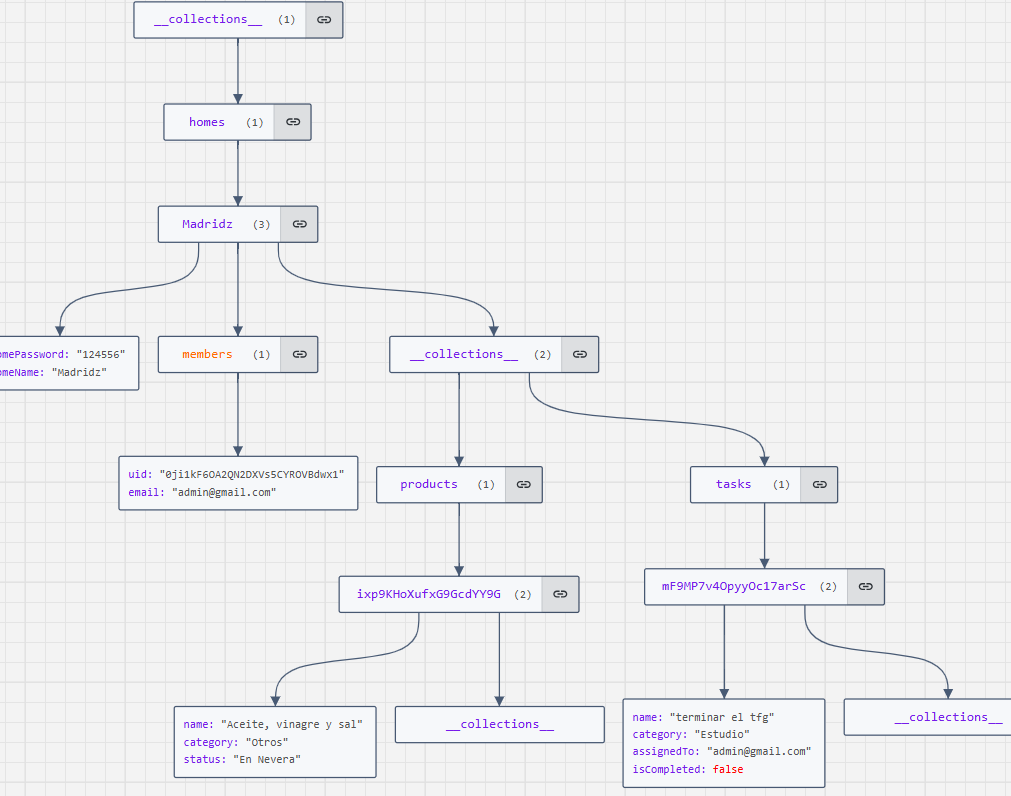
\includegraphics[width=1.1\textwidth, height=0.8\textheight]{TFG/img/json.png}
    \caption{Estructura de datos visualizada en JSON.}
    \label{fig:json_structure}
\end{figure}
        \end{itemize}

                

     

   \section{Planificaci\'on Completa del Proyecto}

\subsection{Planteamiento Principal}

\begin{table}[H]
\centering
\begin{tabular}{|l|l|}
    \hline
    \textbf{Clave} & \textbf{Funcionalidades} \\ \hline
     & Inicio de la Aplicaci\'on \\ \hline
    F1 & Nombre de la aplicaci\'on \\ \hline
    F2 & Logo de la aplicaci\'on \\ \hline
    F3 & Investigaci\'on de herramientas \\ \hline
     & Dise\~no de Aplicaci\'on \\ \hline
    F4 & Diagrama de Gantt \\ \hline
    F5 & Diagrama de flujo \\ \hline
    F6 & Dise\~no en el front \\ \hline
     & Desarrollo \\ \hline
    F7 & Desarrollo de usuarios \\ \hline
    F8 & Desarrollo de grupo de hogar \\ \hline
    F9 & Desarrollo del to-do \\ \hline
    F10 & Desarrollo de gesti\'on de nevera \\ \hline
    F11 & Desarrollo de ajustes \\ \hline
     & Implementaci\'on en Firebase \\ \hline
    F12 & Implementaci\'on de Firebase en usuarios \\ \hline
    F13 & Implementaci\'on de Firebase en grupo de hogar \\ \hline
    F14 & Implementaci\'on de Firebase en el to-do \\ \hline
    F15 & Implementaci\'on de Firebase en la gesti\'on de nevera \\ \hline
    F16 & Implementaci\'on de Firebase en ajustes \\ \hline
     & Pruebas y Seguridad \\ \hline
    F17 & Implementaci\'on de mejoras \\ \hline
    F18 & Comprobaci\'on del funcionamiento en Android e iOS \\ \hline
     & Documentaci\'on \\ \hline
    F19 & Documentaci\'on en PDF \\ \hline
    F20 & Presentaci\'on en PowerPoint \\ \hline
\end{tabular}
\caption{Tabla de Funcionalidades}
\label{tab:funcionalidades}
\end{table}

\clearpage

\subsubsection{Inicio de la Aplicaci\'on}
\begin{itemize}
    \item \textbf{F1: Nombre de la aplicaci\'on}  
    Determinar y definir un nombre distintivo para la aplicaci\'on que sea memorable y representativo de su funci\'on principal.
    
    \item \textbf{F2: Logo de la aplicaci\'on}  
    Dise\~nar un logotipo que identifique visualmente la aplicaci\'on, alineado con la tem\'atica y estilo de la interfaz.
    
    \item \textbf{F3: Investigaci\'on de herramientas}  
    Explorar y seleccionar herramientas de desarrollo, lenguajes, dise\~no y bases de datos que mejor se adapten al proyecto.
\end{itemize}

\subsubsection{Dise\~no de la Aplicaci\'on}
\begin{itemize}
    \item \textbf{F4: Diagrama de Gantt}  
    Crear un cronograma que detalle las fases del proyecto, incluyendo las tareas y sus tiempos de ejecuci\'on.
    
    \item \textbf{F5: Diagrama de flujo}  
    Dise\~nar un esquema que muestre el flujo l\'ogico y funcional de la aplicaci\'on, facilitando la comprensi\'on de su estructura.
    
    \item \textbf{F6: Dise\~no en el front}  
    Crear los prototipos o bocetos de las pantallas de la aplicaci\'on, definiendo la est\'etica y experiencia de usuario (UX/UI).
\end{itemize}

\subsubsection{Desarrollo}
\begin{itemize}
    \item \textbf{F7: Desarrollo de usuarios}  
    Programar la funcionalidad que permita gestionar el registro, inicio de sesi\'on y perfiles de usuario.
    
    \item \textbf{F8: Desarrollo de grupo de hogar}  
    Crear la funci\'on que gestione la creaci\'on y administraci\'on de grupos, vinculados a hogares o grupos familiares.
    
    \item \textbf{F9: Desarrollo del to-do}  
    Implementar una funcionalidad para gestionar listas de tareas pendientes (to-do), permitiendo agregar, editar y completar tareas.
    
    \item \textbf{F10: Desarrollo de gesti\'on de nevera}  
    Programar una herramienta que permita al usuario registrar y organizar los productos almacenados en su nevera, utilizando un enfoque visual.
    
    \item \textbf{F11: Desarrollo de ajustes}  
    Implementar una secci\'on donde los usuarios puedan personalizar la configuraci\'on de la aplicaci\'on seg\'un sus preferencias.
\end{itemize}

\subsubsection{Implementaci\'on en Firebase}
\begin{itemize}
    \item \textbf{F12: Implementaci\'on de Firebase en usuarios}  
    Integrar Firebase para almacenar y sincronizar datos de los usuarios, como credenciales y perfiles.
    
    \item \textbf{F13: Implementaci\'on de Firebase en grupo de hogar}  
    Configurar Firebase para gestionar la informaci\'on y datos de los grupos de hogar, permitiendo colaboraci\'on entre usuarios.
    
    \item \textbf{F14: Implementaci\'on de Firebase en el to-do}  
    Usar Firebase para guardar y sincronizar las listas de tareas en tiempo real.
    
    \item \textbf{F15: Implementaci\'on de Firebase en la gesti\'on de nevera}  
    Aplicar Firebase para registrar y sincronizar la informaci\'on sobre los productos disponibles en la nevera.
    
    \item \textbf{F16: Implementaci\'on de Firebase en ajustes}  
    Sincronizar la configuraci\'on personalizada de los usuarios a trav\'es de Firebase para que se mantenga en todos los dispositivos.
\end{itemize}

\subsubsection{Pruebas y Seguridad}
\begin{itemize}
    \item \textbf{F17: Implementaci\'on de mejoras}  
    Revisar y ajustar las funcionalidades para optimizar el rendimiento y corregir posibles errores o deficiencias.
    
    \item \textbf{F18: Comprobaci\'on del funcionamiento en Android e iOS}  
    Realizar pruebas exhaustivas para verificar que la aplicaci\'on funcione correctamente en ambas plataformas, detectando errores de compatibilidad.
\end{itemize}

\subsubsection{Documentaci\'on}
\begin{itemize}
    \item \textbf{F19: Documentaci\'on en PDF}  
    Generar un documento formal que explique el desarrollo de la aplicaci\'on, incluyendo an\'alisis, dise\~no, implementaci\'on y pruebas.
    
    \item \textbf{F20: Presentaci\'on en PowerPoint}  
    Crear una presentaci\'on visual para exponer el proyecto, destacando sus funcionalidades y caracter\'isticas principales.
\end{itemize}

\addcontentsline{lof}{section}{Diagramas}

\begin{figure}[H]
    \begin{ganttchart}[
        x unit=0.120cm, % distancia entre cada unidad horizontal (días).
        y unit chart=0.5cm, % altura de cada unidad vertical.
        y unit title=0.7cm, % altura de las filas de títulos.
        title height=1, % separación entre una fila de títulos y otra (1 = ninguna separación).
        hgrid, % dibujar las separaciones verticales.
        vgrid={*6{draw=none}, dotted}, % dibujar las separaciones verticales en intervalos semanales.
        bar/.append style={fill=white}, % barras de color blanco por defecto.
        group peaks width=3,
        group peaks tip position=0.5,
        group peaks height=.1, % distintos parámetros para el formato de los grupos.
        time slot format=isodate, % formato de las fechas.
    ] {2024-09-26}{2024-12-15} % inicio y final del eje temporal (año-mes-día).

    % Títulos:
    \gantttitle{Diagrama de Gantt: TaskTracer}{81} \\ % Título centrado y extendido
    \gantttitlecalendar{year, month=shortname} \\ 
    \gantttitlecalendar[title height=2, title label node/.append style={rotate=90}]{week} \\
    \gantttitle[title/.style={opacity=0}]{}{364} \\ 

    % Grupos y tareas:
    \ganttgroup{Inicio de la Aplicaci\'on}{2024-09-26}{2024-09-29} \\
    \ganttbar[bar/.append style={fill=blue!20}]{F1  \Large {\CheckedBox}}{2024-09-26}{2024-09-26} \\
    \ganttbar[bar/.append style={fill=blue!20}]{F2  \Large {\CheckedBox}}{2024-09-27}{2024-09-28} \\
    \ganttbar[bar/.append style={fill=blue!20}]{F3  \Large {\CheckedBox}}{2024-09-28}{2024-09-29} \\

    \ganttgroup{Dise\~no de Aplicaci\'on}{2024-09-30}{2024-10-16} \\
    \ganttbar[bar/.append style={fill=orange!50}]{F4 \Large {\CheckedBox}}{2024-09-30}{2024-10-04} \\
    \ganttbar[bar/.append style={fill=orange!50}]{F5 \Large {\CheckedBox}}{2024-10-05}{2024-10-08} \\
    \ganttbar[bar/.append style={fill=orange!50}]{F6 \Large {\CheckedBox}}{2024-10-12}{2024-10-16} \\

    \ganttgroup{Desarrollo}{2024-10-17}{2024-11-20} \\
    \ganttbar[bar/.append style={fill=green!50}]{F7 \Large {\CheckedBox}}{2024-10-17}{2024-10-22} \\
    \ganttbar[bar/.append style={fill=green!50}]{F8 \Large {\CheckedBox}}{2024-10-23}{2024-10-28} \\
    \ganttbar[bar/.append style={fill=green!50}]{F9  \Large {\CheckedBox}}{2024-10-29}{2024-11-03} \\
    \ganttbar[bar/.append style={fill=green!50}]{F10 \Large {\CheckedBox}}{2024-11-04}{2024-11-09} \\
    \ganttbar[bar/.append style={fill=green!50}]{F11 \Large {\CheckedBox}}{2024-11-10}{2024-11-15} \\ 

    \ganttgroup{Implementaci\'on en Firebase}{2024-11-15}{2024-12-01} \\
    \ganttbar[bar/.append style={fill=blue!50}]{F12 \Large {\CheckedBox}}{2024-11-15}{2024-11-17} \\
    \ganttbar[bar/.append style={fill=blue!50}]{F13 \Large {\CheckedBox}}{2024-11-17}{2024-11-22} \\
    \ganttbar[bar/.append style={fill=blue!50}]{F14 \Large {\CheckedBox}}{2024-11-22}{2024-11-27} \\
    \ganttbar[bar/.append style={fill=blue!50}]{F15 \Large {\CheckedBox}}{2024-11-27}{2024-11-30} \\
    \ganttbar[bar/.append style={fill=blue!50}]{F16 \Large {\CheckedBox}}{2024-11-30}{2024-12-01} \\

    \ganttgroup{Pruebas y Seguridad}{2024-12-01}{2024-12-10} \\
    \ganttbar[bar/.append style={fill=red!50}]{F17 \Large {\XBox}}{2024-12-01}{2024-12-10} \\ 
    \ganttbar[bar/.append style={fill=red!50}]{F18 \Large {\XBox}}{2024-12-10}{2024-12-12} \\ 

    \ganttgroup{Documentaci\'on}{2024-11-20}{2024-12-15} \\
    \ganttbar[bar/.append style={fill=red!30}]{F19 \Large {\XBox}}{2024-11-20}{2024-12-15} \\ 
    \ganttbar[bar/.append style={fill=red!30}]{F20 \Large {\XBox}}{2024-12-09}{2024-12-15} \\ 

    \end{ganttchart}
    \caption{Diagrama de Gantt de TaskTracer}
    \label{fig:gantt}
\end{figure}



  \subsection{Mejoras o Ideas para Implementar en un Futuro}

\begin{table}[H]
\centering
\begin{tabular}{|l|p{0.7\textwidth}|c|}
    \hline
    \textbf{Pantalla/Actividad} & \textbf{Mejoras o Ideas Futuras} & \textbf{Estado} \\ \hline
    
    \textbf{LoginScreen} & 
    \begin{tabular}[t]{@{}l@{}}
        - Opci\'on de mostrar contrase\~na. \\
        - Inicio de sesi\'on con Gmail. \\
        - Deshabilitar botones si no hay conexi\'on a internet.
    \end{tabular} & 
    En planificaci\'on \\ \hline
    
    \textbf{Register} & 
    \begin{tabular}[t]{@{}l@{}}
        - Opci\'on de mostrar contrase\~na. \\
        - Registro con Gmail. \\
        - Deshabilitar botones si no hay conexi\'on a internet.
    \end{tabular} & 
    En planificaci\'on \\ \hline
    
    \textbf{GrupoScreen} & 
    \begin{tabular}[t]{@{}l@{}}
        - Detectar si el usuario ya tiene un domicilio registrado y, de ser as\'i, \\
          redirigir directamente al \textit{Home Activity}.
    \end{tabular} & 
    Pendiente \\ \hline
    
    \textbf{To-Do} & 
    \begin{tabular}[t]{@{}l@{}}
        - Actualizar las tareas al arrastrar hacia abajo. \\
        - A\~nadir la posibilidad de incluir una descripci\'on\\ al presionar en el medio de la tarea.
    \end{tabular} & 
    En planificaci\'on \\ \hline
    
    \textbf{Gesti\'on de Nevera} & 
    \begin{tabular}[t]{@{}l@{}}
        - Agregar productos mediante una opci\'on que utilice la\\ API de Mercadona. \\
        - A\~nadir opciones de editar y eliminar productos.
    \end{tabular} & 
    Pendiente \\ \hline
    
    \textbf{Gesti\'on de Ajustes} & 
    \begin{tabular}[t]{@{}l@{}}
        - Permitir al usuario cargar una imagen como foto de perfil al \\ hacer clic 
          en su foto de usuario.
    \end{tabular} & 
    Pendiente \\ \hline
\end{tabular}
\caption{Mejoras o ideas para implementar en el futuro}
\label{tab:mejoras}
\end{table}

\clearpage


        \addcontentsline{lof}{section}{Analisis y Diseño}
\section{An\'alisis y Dise\~no}

\subsection{Navegaci\'on por pantallas}
A continuaci\'on, iremos viendo la navegaci\'on y descripci\'on de cada pantalla para obtener una visi\'on general de la aplicaci\'on.

\subsubsection{Archivo Principal (\texttt{main.dart})}
\begin{itemize}
    \item \textbf{Descripci\'on}: 
    Este archivo act\'ua como punto de entrada para la aplicaci\'on. Inicializa Firebase, configura los temas visuales y gestiona la verificaci\'on del estado de autenticaci\'on del usuario para redirigirlo a la pantalla correspondiente.

    \item \textbf{Requisitos}: 
    \begin{itemize}
        \item Firebase debe estar configurado e inicializado correctamente en el proyecto.
        \item Las pantallas de bienvenida (\texttt{WelcomeScreen}) y principal (\texttt{HomeScreen}) deben estar implementadas.
        \item La clase \texttt{DefaultFirebaseOptions} debe estar configurada con las credenciales de Firebase.
    \end{itemize}

    \item \textbf{Componentes principales}:
    \begin{itemize}
        \item \textbf{Clase \texttt{MyApp}}:
        \begin{itemize}
            \item Define el tema global de la aplicaci\'on.
            \item Especifica la pantalla inicial basada en el estado de autenticaci\'on mediante el widget \texttt{AuthCheck}.
        \end{itemize}

        \item \textbf{Widget \texttt{AuthCheck}}:
        \begin{itemize}
            \item Escucha los cambios en el estado de autenticaci\'on del usuario a trav\'es de \texttt{FirebaseAuth}.
            \item Redirige al usuario a:
            \begin{itemize}
                \item \texttt{HomeScreen} si el usuario est\'a autenticado.
                \item \texttt{WelcomeScreen} si el usuario no est\'a autenticado.
            \end{itemize}
            \item Muestra un indicador de carga mientras se verifica el estado de autenticaci\'on.
        \end{itemize}
    \end{itemize}

    \item \textbf{Flujo de la Aplicaci\'on}:
    \begin{itemize}
        \item La aplicaci\'on se inicializa mediante \texttt{Firebase.initializeApp}.
        \item Se verifica el estado de autenticaci\'on del usuario:
        \begin{itemize}
            \item Si el usuario est\'a autenticado, es redirigido a \texttt{HomeScreen}.
            \item Si el usuario no est\'a autenticado, es redirigido a \texttt{WelcomeScreen}.
        \end{itemize}
    \end{itemize}
\end{itemize}


\clearpage

\subsubsection{Pantalla de Arranque (\texttt{SplashScreen})}
\begin{itemize}
    \item \textbf{Descripci\'on}: 
    Es la primera pantalla que se muestra cuando se abre la aplicaci\'on. Contiene el logotipo de la aplicaci\'on.

    \item \textbf{Navegaci\'on}: 
    Esta pantalla lleva al usuario, una vez han transcurrido tres segundos, a la pantalla de bienvenida (\texttt{WelcomeScreen}).
\end{itemize}

\begin{figure}[H]
    \centering
    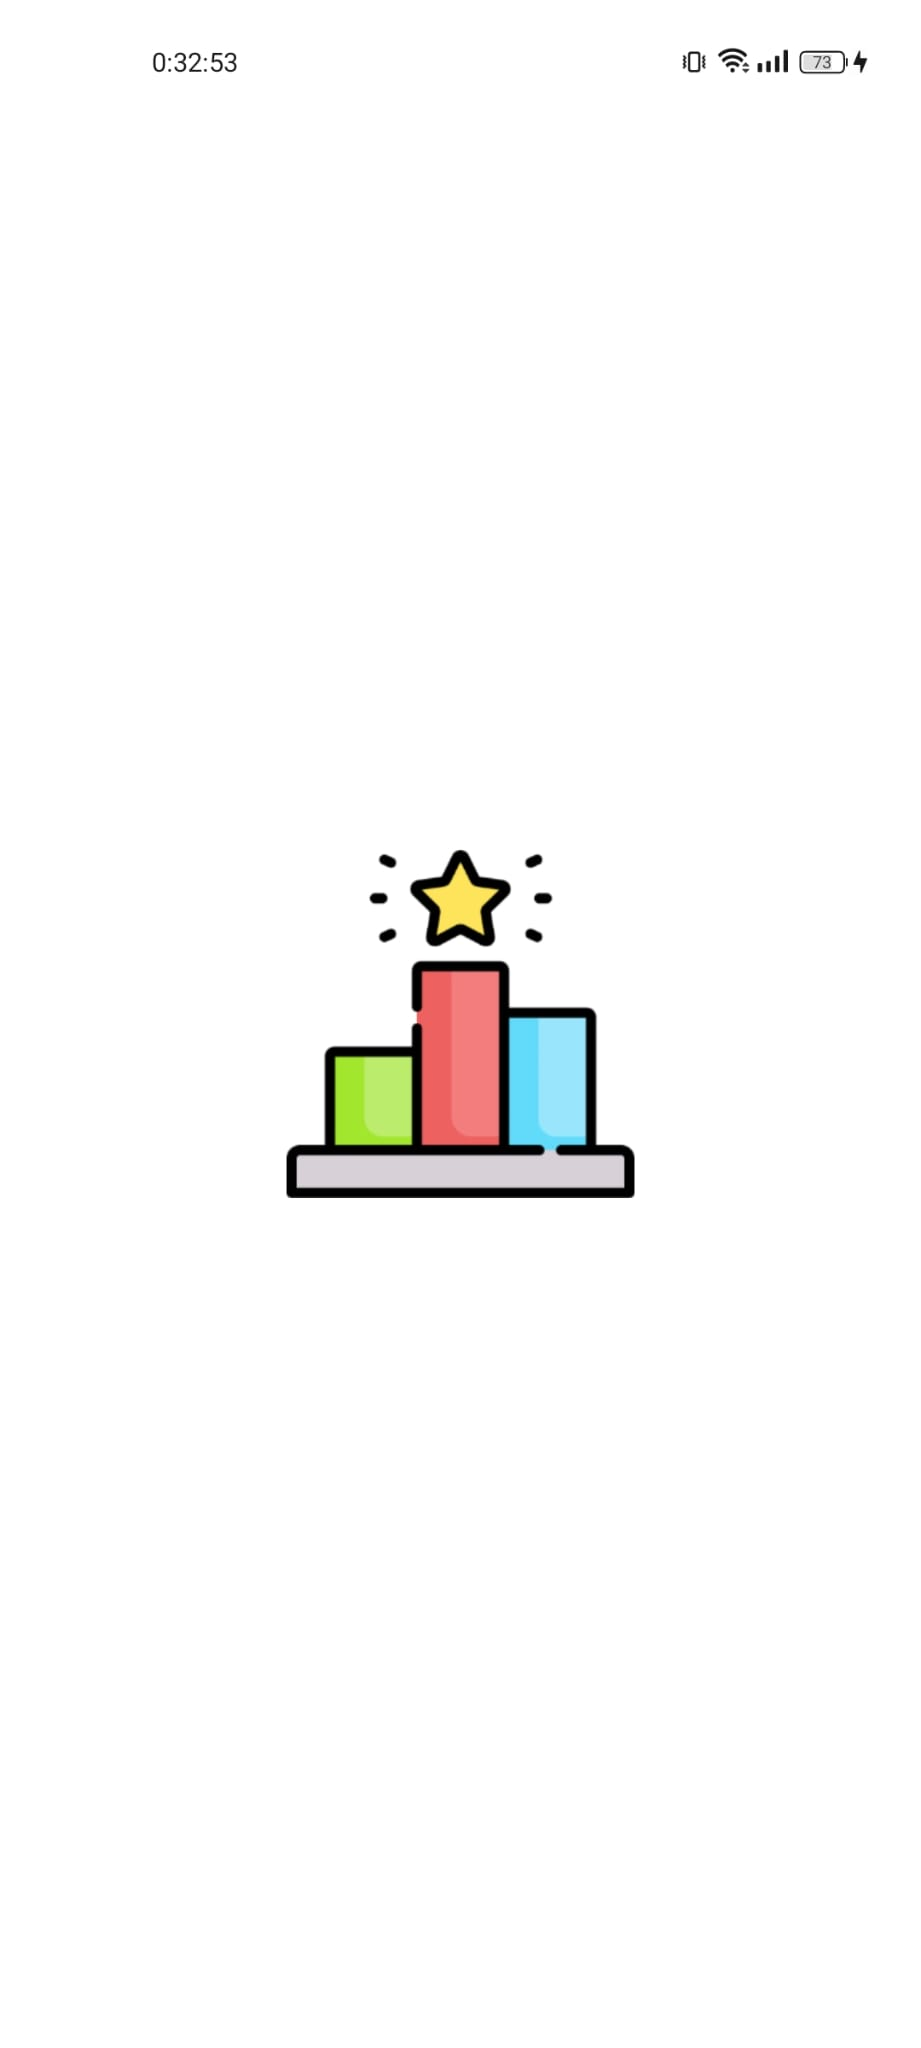
\includegraphics[width=0.3\textwidth]{TFG/img/img/splaah.jpeg}
    \caption{Pantalla de Arranque (\texttt{SplashScreen}).}
    \label{fig:splash_screen}
\end{figure}

\clearpage

\subsubsection{Pantalla de Bienvenida (\texttt{WelcomeScreen})}
\begin{itemize}
    \item \textbf{Descripci\'on}: 
    La pantalla de bienvenida es la primera interacci\'on del usuario despu\'es de la pantalla de arranque. Incluye una imagen representativa, un mensaje de bienvenida y una breve descripci\'on de las principales funcionalidades de la aplicaci\'on. Adem\'as, cuenta con un bot\'on destacado que facilita la navegaci\'on hacia la pantalla de inicio de sesi\'on.
    
    \item \textbf{Navegaci\'on}: 
    El flujo de navegaci\'on de esta pantalla es claro y sencillo. Al pulsar el bot\'on \texttt{Comenzar}, el usuario es redirigido autom\'aticamente a la pantalla de inicio de sesi\'on (\texttt{LoginScreen}).

    \item \textbf{Listado de contenidos}: 
    \begin{itemize}
        \item \textbf{Imagen representativa}: Una imagen ubicada en la parte superior que refuerza la identidad visual de la aplicaci\'on.
        \item \textbf{Mensaje de bienvenida}: Un texto amigable que recibe al usuario y destaca el nombre de la aplicaci\'on.
        \item \textbf{Descripci\'on de funcionalidades}: Un breve texto que informa al usuario sobre las principales utilidades de la aplicaci\'on, como la organizaci\'on de tareas y la gesti\'on de productos en la nevera.
        \item \textbf{Bot\'on de acci\'on \texttt{Comenzar}}: Un bot\'on claramente visible que permite al usuario avanzar a la pantalla de inicio de sesi\'on (\texttt{LoginScreen}).
    \end{itemize}
\end{itemize}

\begin{figure}[H]
    \centering
    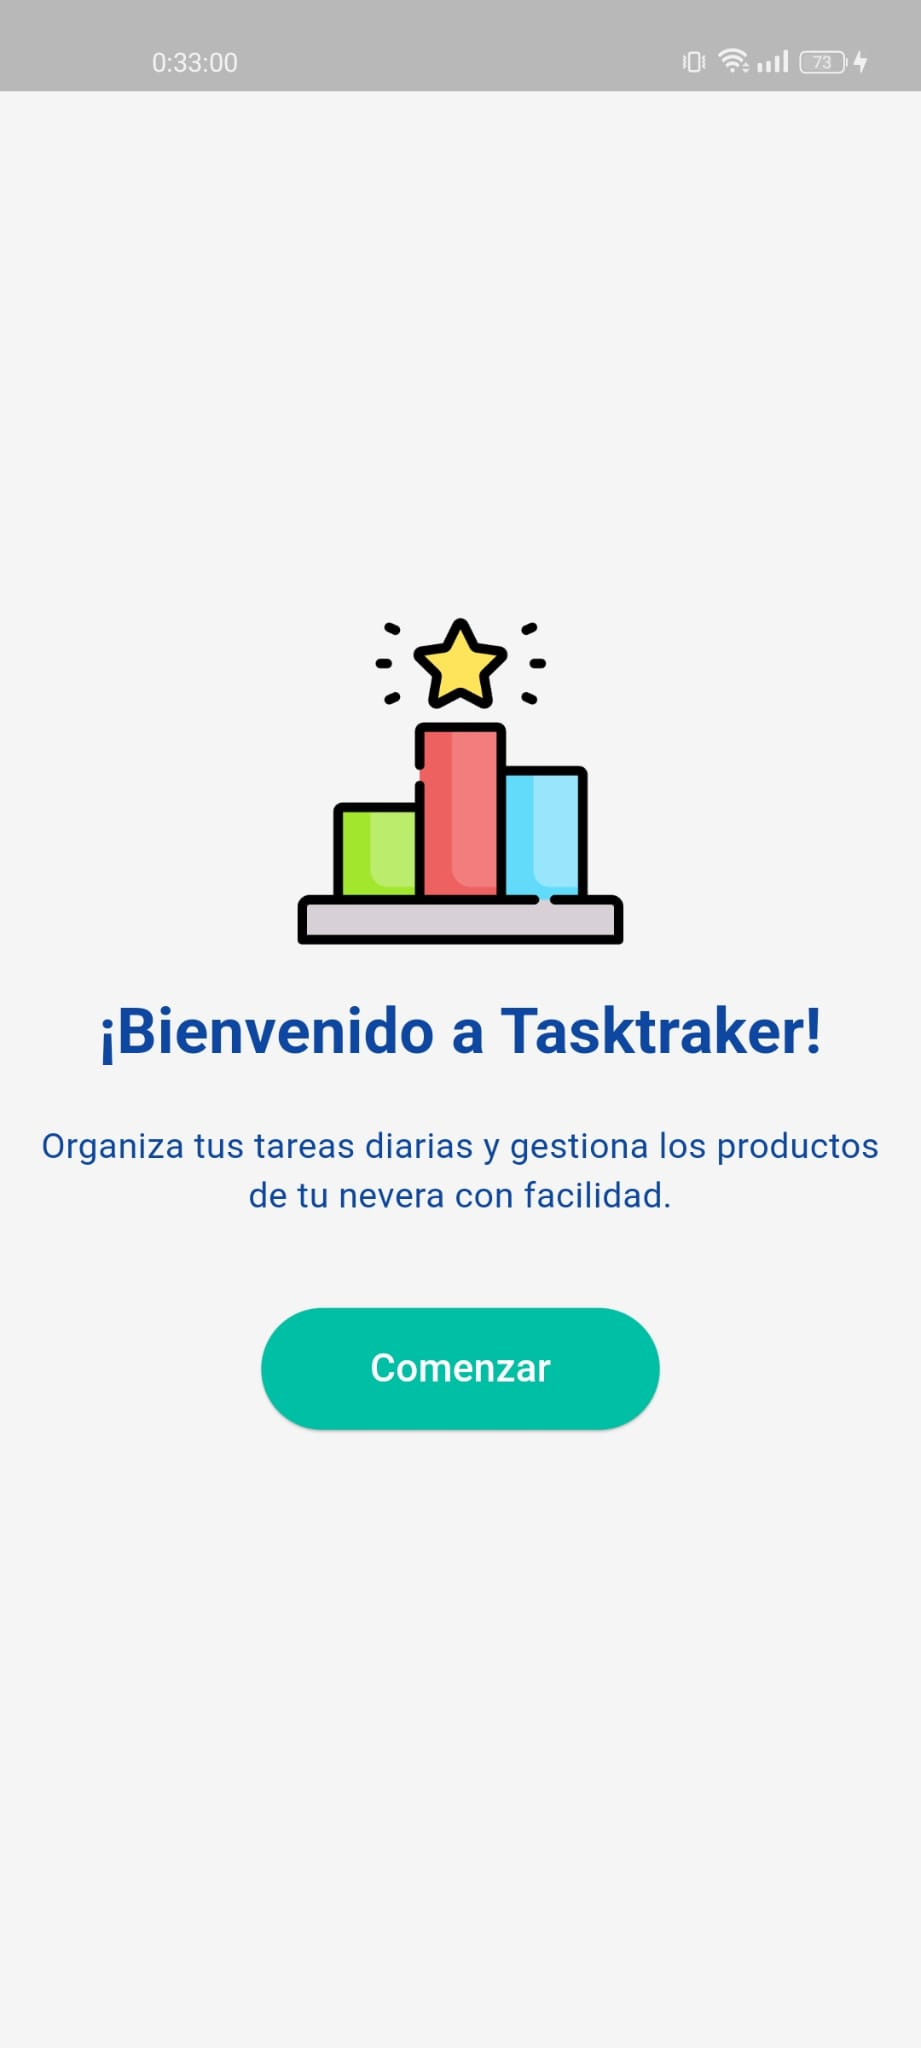
\includegraphics[width=0.3\textwidth]{TFG/img/img/welcome.jpeg}
    \caption{Pantalla de Bienvenida (\texttt{WelcomeScreen}).}
    \label{fig:welcome_screen}
\end{figure}

\clearpage


\subsubsection{Pantalla de Inicio de Sesi\'on (\texttt{LoginScreen})}
\begin{itemize}
    \item \textbf{Descripci\'on}: 
    La pantalla de inicio de sesi\'on permite a los usuarios acceder a su cuenta proporcionando un correo electr\'onico y contrase\~na previamente registrados. Incluye validaciones de los campos ingresados, un indicador de carga durante el proceso de inicio de sesi\'on y un mensaje de error en caso de credenciales incorrectas. Adem\'as, ofrece un enlace para redirigir a la pantalla de registro en caso de no tener cuenta.

    \item \textbf{Requisitos}: 
    \begin{itemize}
        \item El usuario debe ingresar un correo electr\'onico registrado y v\'alido.
        \item La contrase\~na debe coincidir con la registrada previamente.
        \item El correo electr\'onico debe estar verificado.
    \end{itemize}

    \item \textbf{Navegaci\'on}: 
    Una vez completado el inicio de sesi\'on, el usuario es redirigido a la pantalla principal (\texttt{GroupScreen}). Si el correo no est\'a verificado, se muestra un mensaje y se redirige nuevamente a la pantalla de inicio de sesi\'on. Tambi\'en ofrece un enlace a la pantalla de registro (\texttt{RegistrarScreen}) para los usuarios que no tienen cuenta.

    \item \textbf{Listado de contenidos}: 
    \begin{itemize}
        \item \textbf{Formulario de inicio de sesi\'on}: Campos para ingresar el correo electr\'onico y la contrase\~na, con validaciones estrictas.
        \item \textbf{Bot\'on "Ingresar"}: Permite enviar la informaci\'on del formulario para autenticar al usuario.
        \item \textbf{Indicador de carga}: Muestra un indicador mientras se procesa el inicio de sesi\'on.
        \item \textbf{Bot\'on "Reg\'istrate"}: Un enlace para los usuarios que no tienen cuenta, que los redirige a la pantalla de registro.
        \item \textbf{Mensaje de error}: Muestra mensajes personalizados en caso de credenciales incorrectas o problemas de verificaci\'on.
    \end{itemize}

    \item \textbf{Funciones principales}:
    \begin{itemize}
        \item \texttt{\_signIn()}:
        \begin{itemize}
            \item Valida los campos del formulario.
            \item Autentica al usuario mediante Firebase Authentication.
            \item Verifica si el correo electr\'onico ha sido validado.
            \item Redirige al usuario a la pantalla principal (\texttt{GroupScreen}).
        \end{itemize}
        \item \texttt{\_buildTextField()}:
        \begin{itemize}
            \item Construye un campo de texto reutilizable con opciones de validaci\'on y visibilidad de contrase\~na.
        \end{itemize}
        \item \texttt{setState()}:
        \begin{itemize}
            \item Controla cambios en el estado de carga y visibilidad de la contrase\~na.
        \end{itemize}
    \end{itemize}
\end{itemize}

\begin{figure}[H]
    \centering
     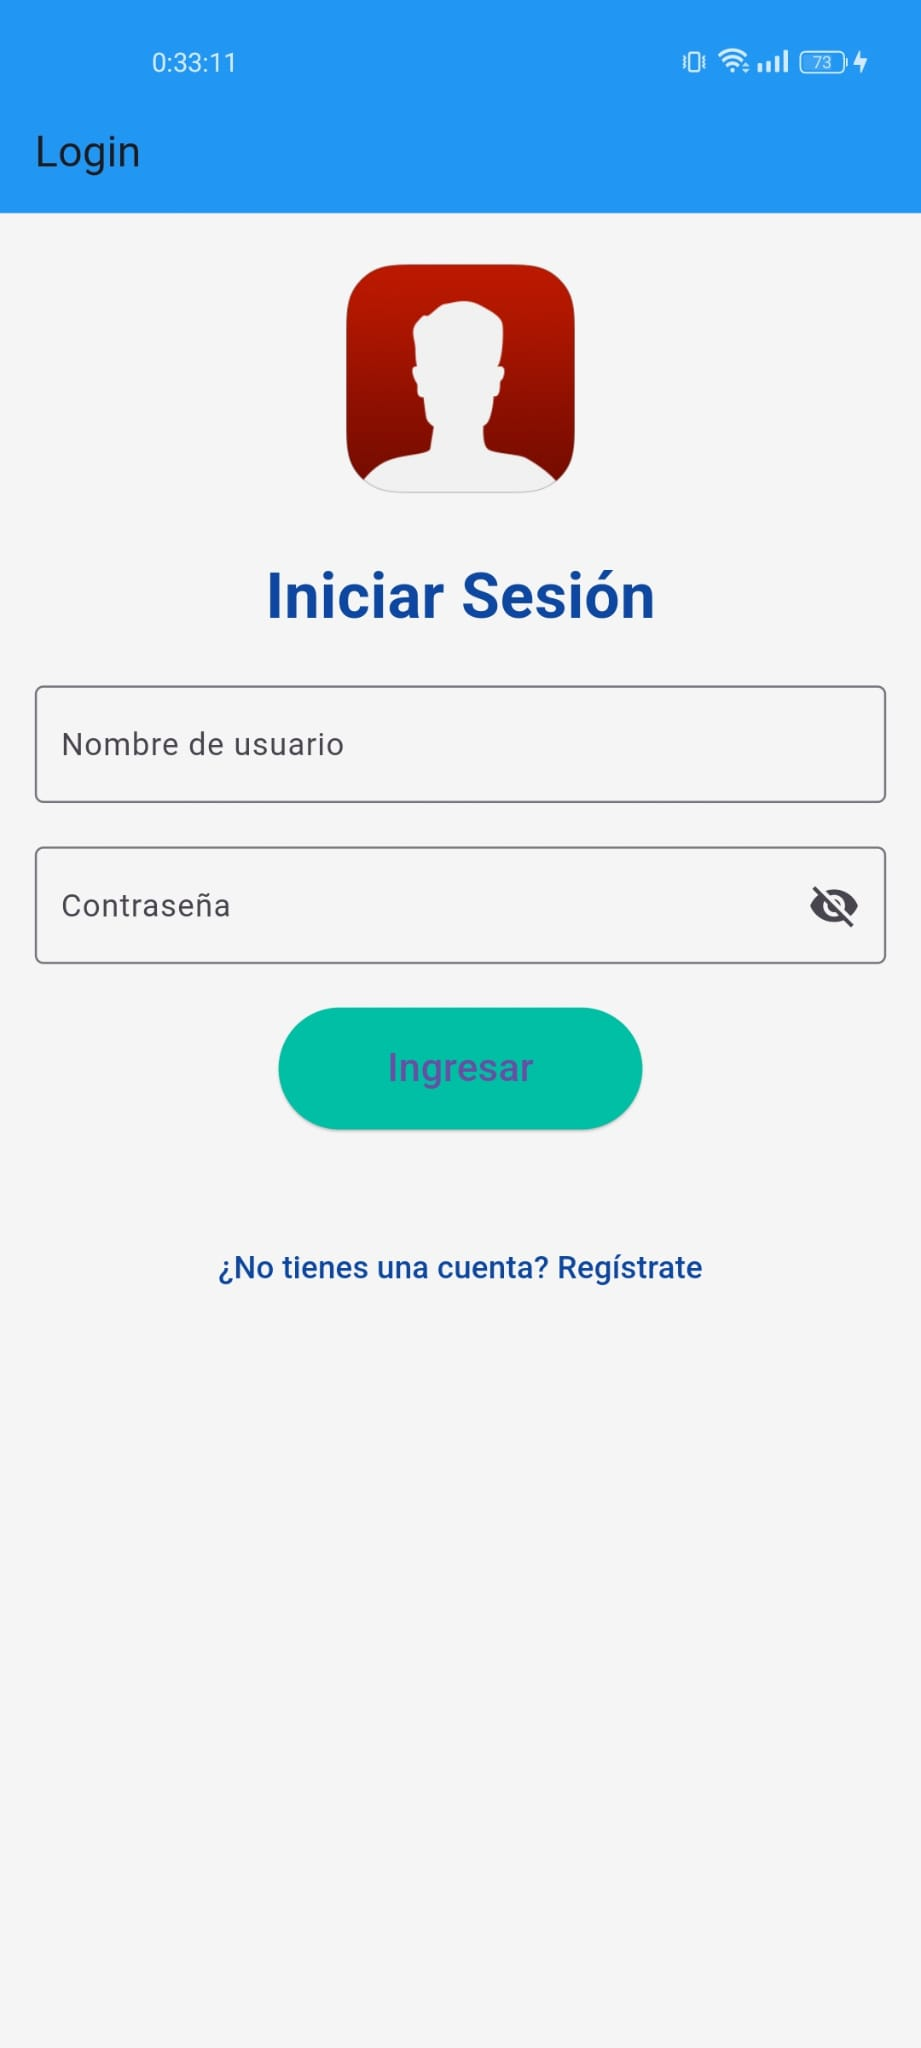
\includegraphics[width=0.3\textwidth]{TFG/img/img/login.jpeg}
    \caption{Pantalla de Inicio de Sesi\'on (\texttt{LoginScreen}).}
    \label{fig:login_screen}
\end{figure}

\clearpage

\subsubsection{Pantalla de Registro (\texttt{RegistrarScreen})}
\begin{itemize}
    \item \textbf{Descripci\'on}: 
    La pantalla de registro permite a los usuarios crear una nueva cuenta proporcionando su correo electr\'onico y contrase\~na. Incluye validaciones de los campos ingresados, instrucciones para crear una contrase\~na segura y usar un correo electr\'onico v\'alido, y un mensaje de confirmaci\'on tras un registro exitoso. Tambi\'en se env\'ia un enlace de verificaci\'on al correo electr\'onico del usuario.

    \item \textbf{Requisitos}: 
    \begin{itemize}
        \item El usuario debe ingresar un correo electr\'onico v\'alido.
        \item La contrase\~na debe tener al menos 8 caracteres, incluyendo may\'usculas, min\'usculas, n\'umeros y caracteres especiales.
        \item Es necesario verificar la cuenta mediante el enlace enviado al correo electr\'onico.
    \end{itemize}

    \item \textbf{Navegaci\'on}: 
    Una vez completado el registro, el usuario es redirigido a la pantalla de verificaci\'on de correo (\texttt{EmailVerificationScreen}). Adem\'as, ofrece la opci\'on de regresar a la pantalla de inicio de sesi\'on.

    \item \textbf{Listado de contenidos}: 
    \begin{itemize}
        \item \textbf{Formulario de registro}: Campos para ingresar el correo electr\'onico y la contrase\~na, con validaciones estrictas.
        \item \textbf{Instrucciones}: Consejos sobre c\'omo crear una contrase\~na segura y usar un correo electr\'onico v\'alido. Estas se muestran de manera opcional mediante un bot\'on de gu\'ia.
        \item \textbf{Bot\'on "Mostrar/Ocultar gu\'ia"}: Un bot\'on interactivo que permite al usuario alternar la visibilidad de las instrucciones para el registro.
        \item \textbf{Bot\'on de acci\'on "Registrarse"}: Permite enviar la informaci\'on del formulario y registrar al usuario.
        \item \textbf{Indicador de carga}: Muestra un indicador mientras se procesa el registro.
        \item \textbf{Bot\'on "Inicia sesi\'on"}: Un enlace para los usuarios que ya tienen cuenta, que los redirige a la pantalla de inicio de sesi\'on.
        \item \textbf{Enlace de verificaci\'on}: Tras el registro exitoso, se env\'ia un correo electr\'onico con un enlace para verificar la cuenta.
    \end{itemize}

    \item \textbf{Funciones principales}:
    \begin{itemize}
        \item \texttt{\_register()}:
        \begin{itemize}
            \item Valida los campos del formulario.
            \item Crea un nuevo usuario con Firebase Authentication.
            \item Env\'ia un enlace de verificaci\'on al correo electr\'onico del usuario.
            \item Redirige al usuario a la pantalla de verificaci\'on de correo.
        \end{itemize}
        \item \texttt{\_buildTextField()}:
        \begin{itemize}
            \item Construye un campo de texto con personalizaci\'on de etiqueta, validaci\'on y visibilidad de contrase\~na.
        \end{itemize}
        \item \texttt{setState()}:
        \begin{itemize}
            \item Controla la visibilidad de la contrase\~na.
            \item Alterna la visibilidad de las instrucciones.
            \item Maneja el estado de carga durante el registro.
        \end{itemize}
    \end{itemize}
\end{itemize}

\begin{figure}[H]
  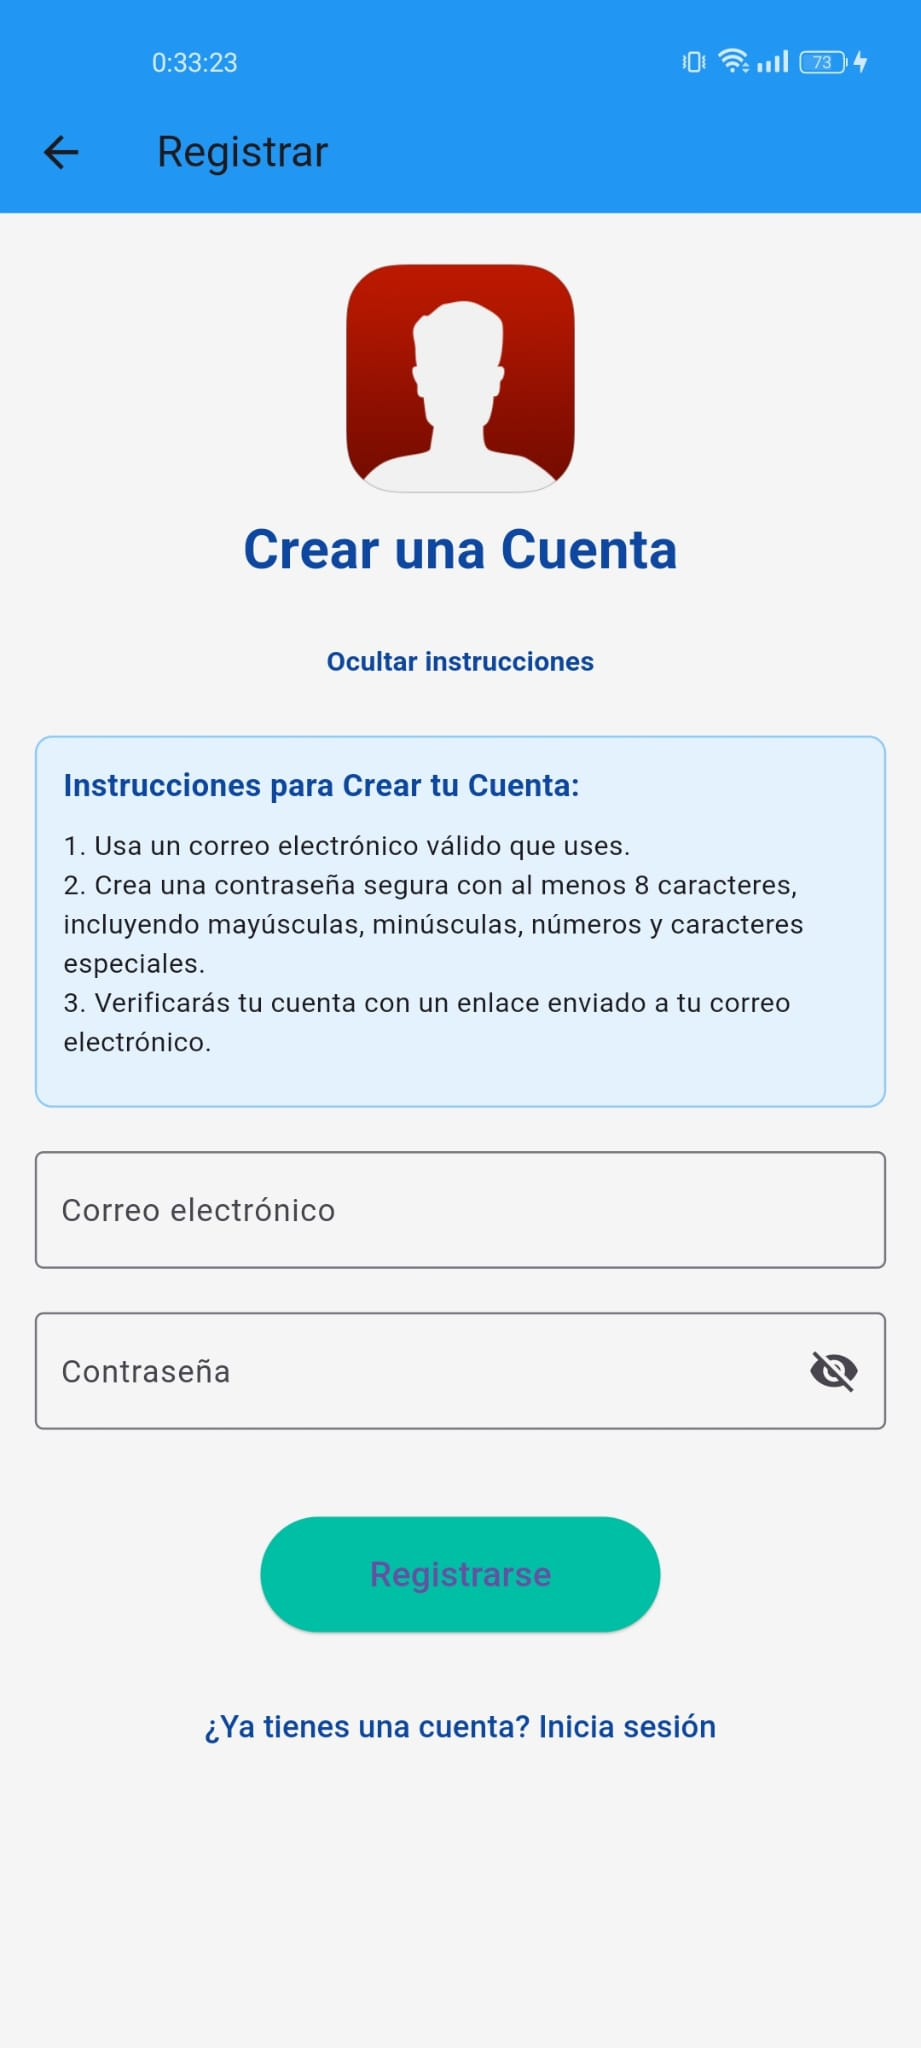
\includegraphics[width=0.3\textwidth]{TFG/img/img/registar1.jpeg}
  
\includegraphics[width=0.3\textwidth]{TFG/img/img/verificacion pantalla.jpeg}
  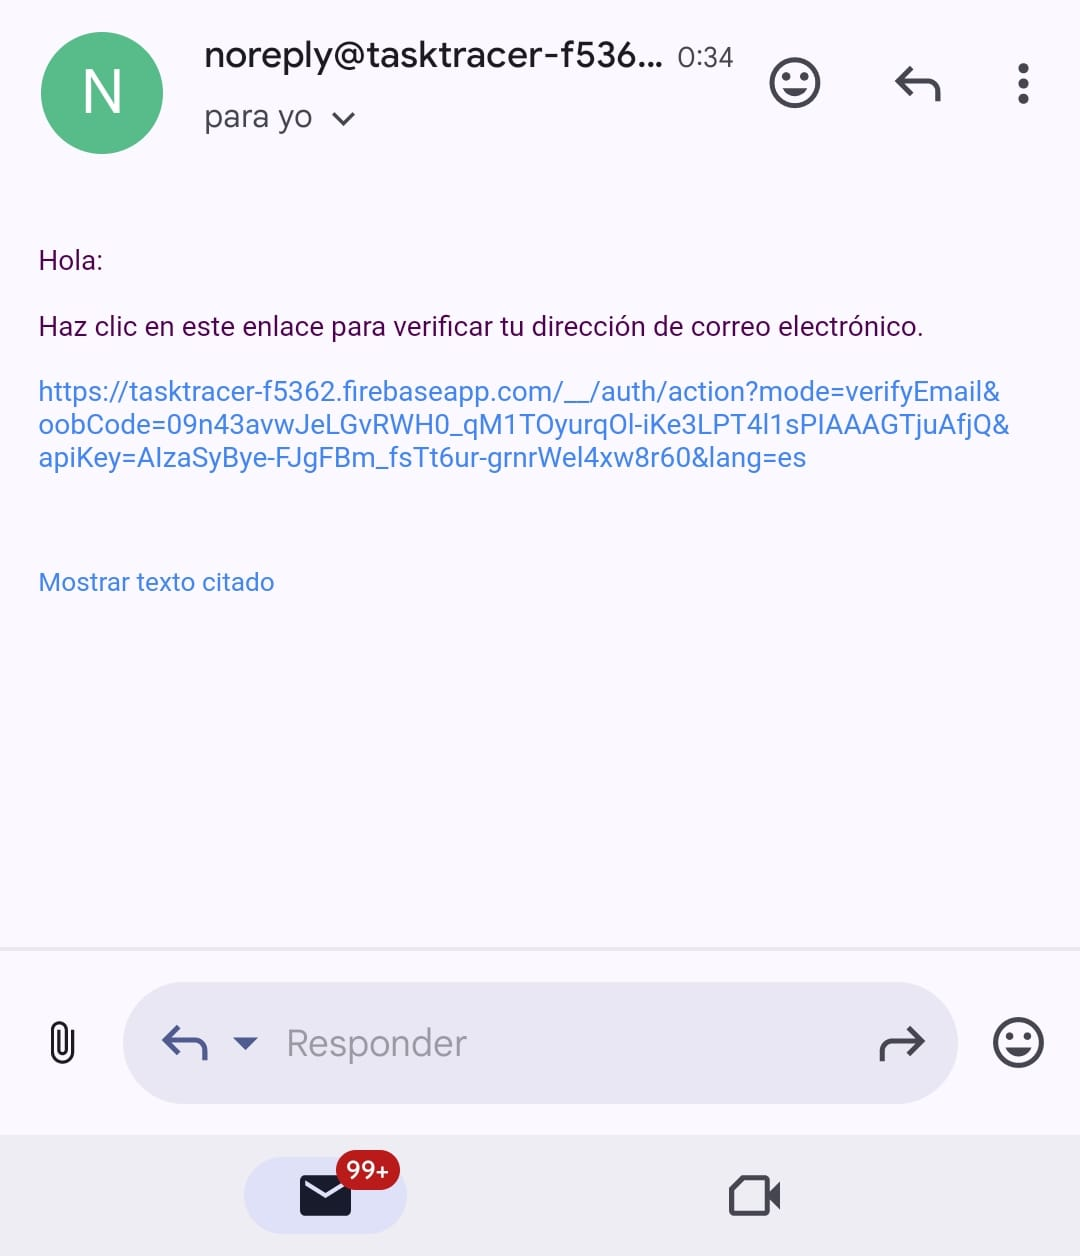
\includegraphics[width=0.3\textwidth]{TFG/img/img/correo.jpeg}
      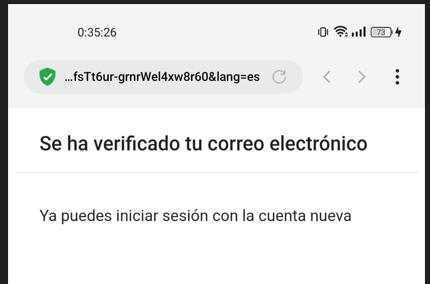
\includegraphics[width=0.3\textwidth]{TFG/img/img/verificacio.png}

    \caption{Pantallas de Registro (\texttt{RegistrarScreen}).}
    \label{fig:registrar_screen}
\end{figure}



\clearpage

\subsubsection{Pantalla de Grupos de Hogar (\texttt{GroupScreen})}
\begin{itemize}
    \item \textbf{Descripci\'on}: 
    La pantalla de grupos de hogar permite a los usuarios gestionar los grupos de los que forman parte, crear nuevos hogares o unirse a un hogar existente. Facilita la conexi\'on de m\'ultiples usuarios a un mismo hogar para compartir y administrar informaci\'on. Un dise\~no intuitivo para facilitar la interacci\'on.

    \item \textbf{Requisitos}: 
    \begin{itemize}
        \item El usuario debe estar autenticado en la aplicaci\'on.
        \item Para crear un hogar, se requiere un nombre \'unico y una contrase\~na.
        \item Para unirse a un hogar, el usuario debe proporcionar el nombre del hogar y la contrase\~na correspondiente.
    \end{itemize}

    \item \textbf{Navegaci\'on}: 
    Tras asociarse a un hogar (ya sea al crear uno o unirse a uno existente), el usuario es redirigido a la pantalla principal (\texttt{HomeScreen}).

    \item \textbf{Listado de contenidos}: 
    \begin{itemize}
        \item \textbf{Formulario para crear un hogar}: Permite ingresar un nombre y una contrase\~na para registrar un nuevo hogar.
        \item \textbf{Formulario para unirse a un hogar}: Permite ingresar el nombre y la contrase\~na de un hogar existente para unirse a \'el.
        \item \textbf{Bot\'on "Crear Hogar"}: Alterna la visibilidad del formulario para registrar un nuevo hogar.
        \item \textbf{Bot\'on "Unirse a Hogar"}: Alterna la visibilidad del formulario para unirse a un hogar existente.
    \end{itemize}

    \item \textbf{Funciones principales}:
    \begin{itemize}
        \item \texttt{\_createHome()}:
        \begin{itemize}
            \item Crea un nuevo hogar en Firebase Firestore con el nombre y contrase\~na proporcionados.
            \item A\~nade al usuario autenticado como miembro del hogar creado.
        \end{itemize}
        \item \texttt{\_joinHome()}:
        \begin{itemize}
            \item Verifica si el hogar y la contrase\~na proporcionados son v\'alidos.
            \item A\~nade al usuario autenticado como miembro del hogar existente.
        \end{itemize}
        \item \texttt{\_buildHomeForm()}:
        \begin{itemize}
            \item Genera un formulario din\'amico para registrar o unirse a un hogar.
            \item Incluye campos de texto con validaci\'on y un bot\'on de acci\'on.
        \end{itemize}
        \item \texttt{setState()}:
        \begin{itemize}
            \item Controla la visibilidad de los formularios (crear o unirse a un hogar).
            \item Alterna la visibilidad de la contrase\~na en los campos correspondientes.
        \end{itemize}
    \end{itemize}
\end{itemize}
 

\begin{figure}[H]
       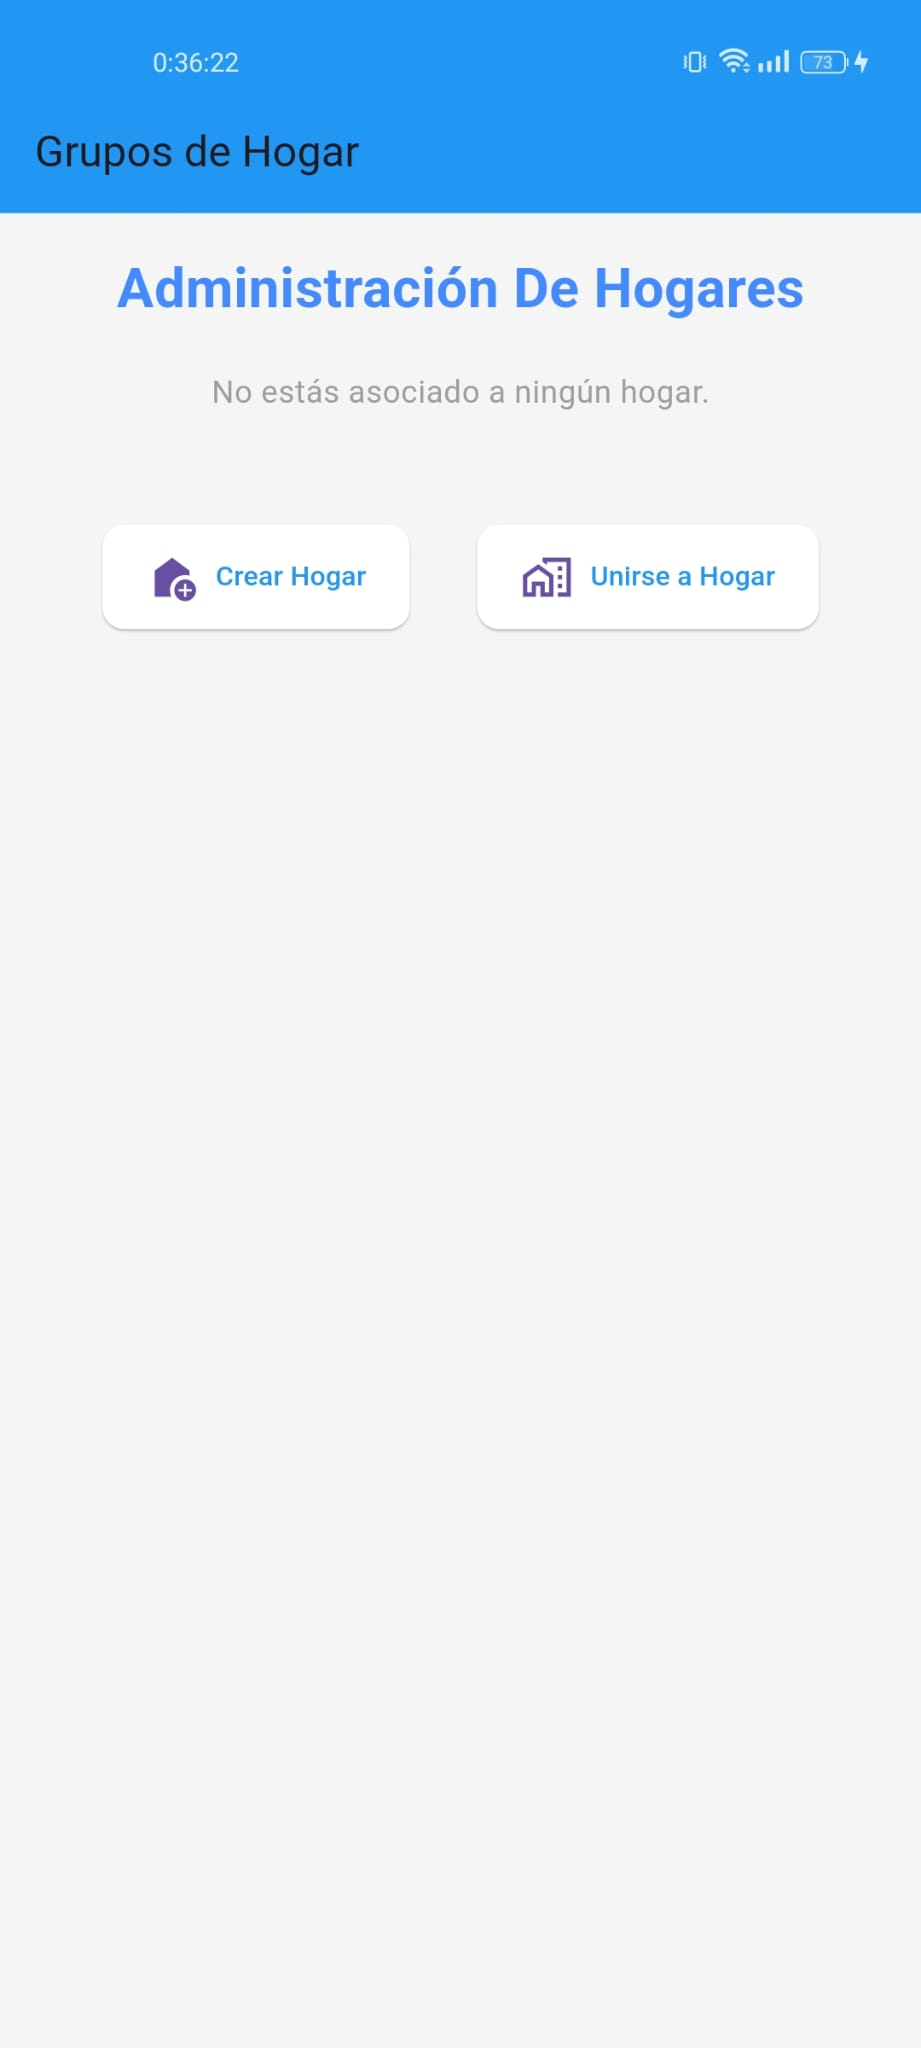
\includegraphics[width=0.3\textwidth]{TFG/img/img/hogar1.jpeg}
     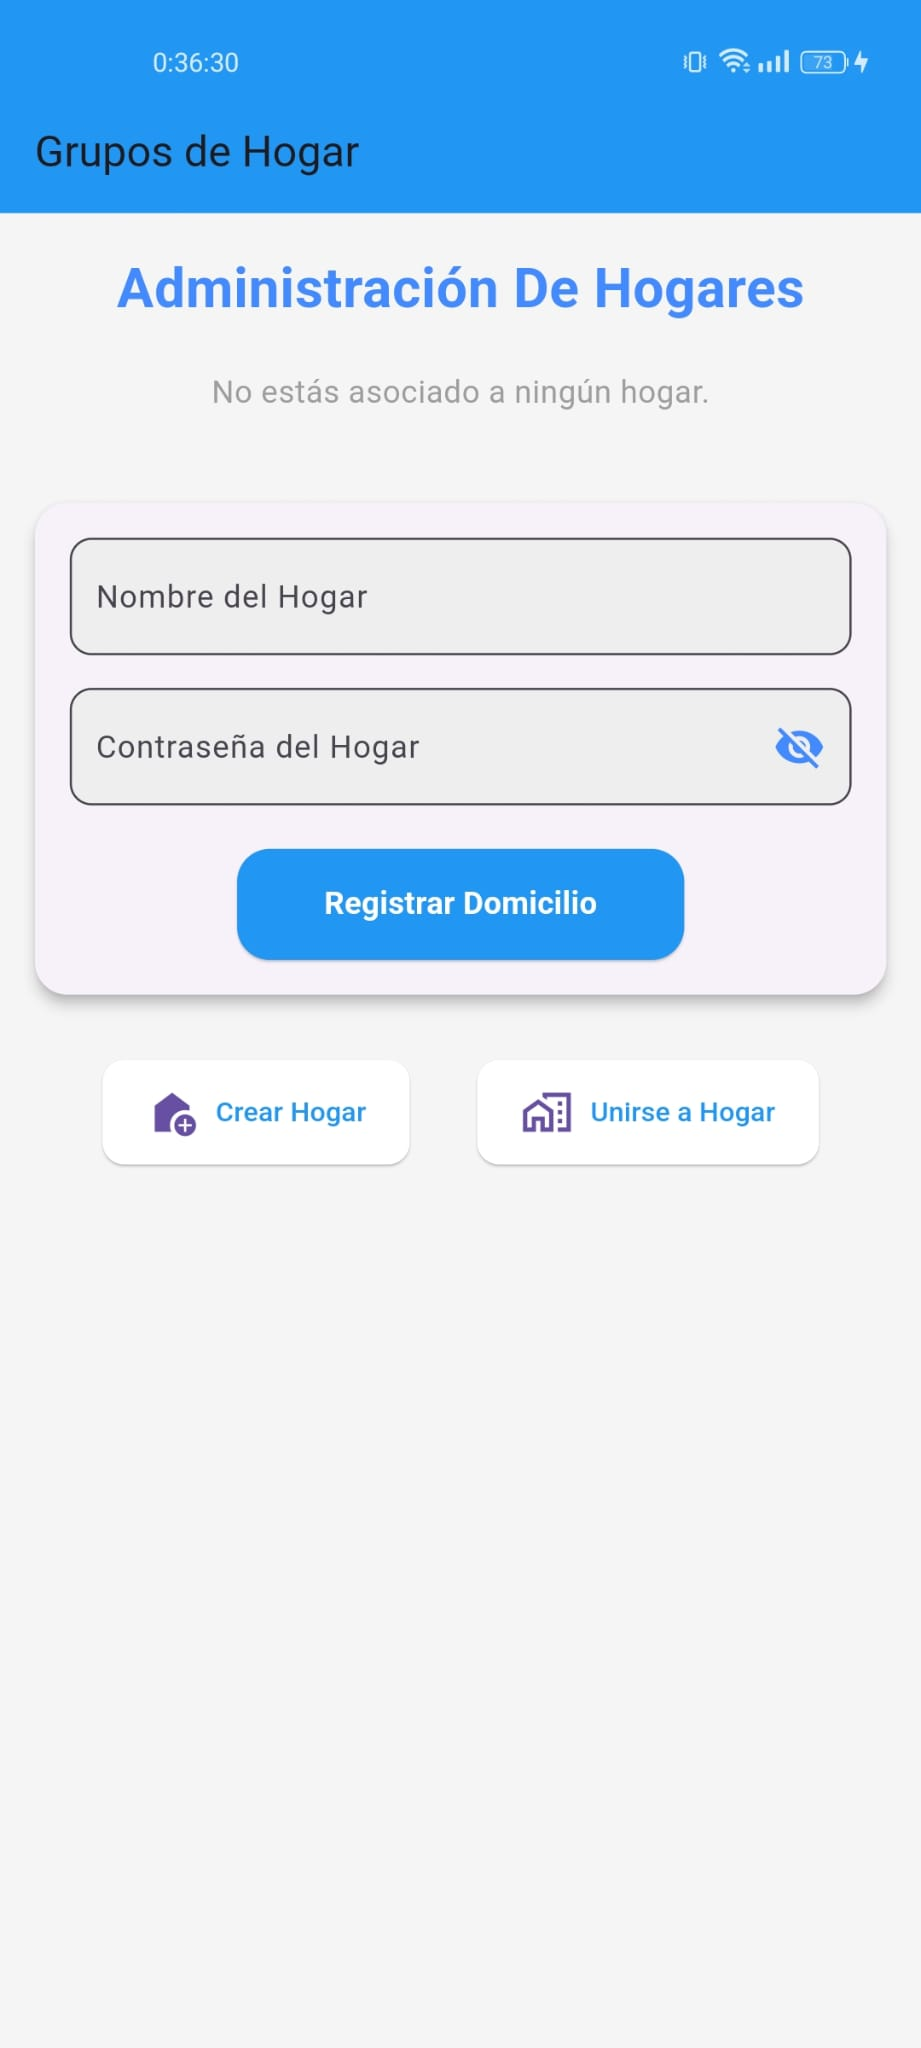
\includegraphics[width=0.3\textwidth]{TFG/img/img/hogar.jpeg}
          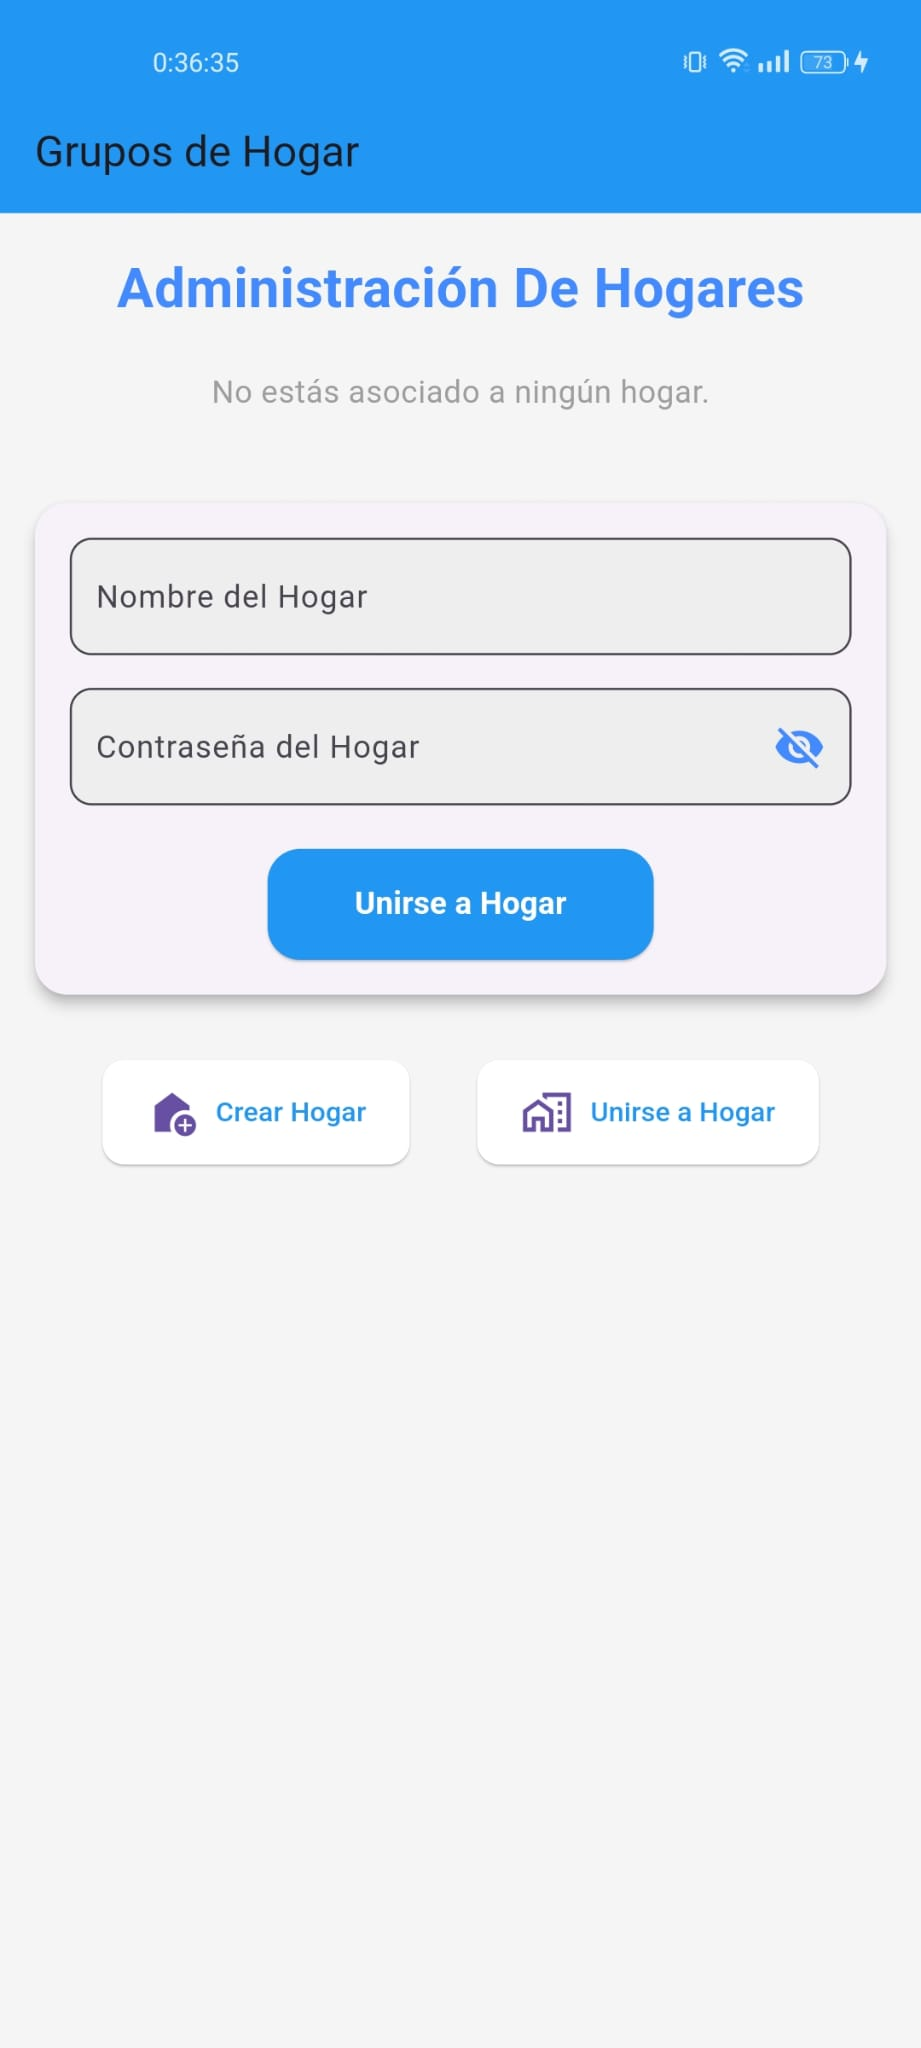
\includegraphics[width=0.3\textwidth]{TFG/img/img/unirse.jpeg}

    \caption{Pantallas de Grupos de Hogar (\texttt{GroupScreen}).}
    \label{fig:group_screen}
\end{figure}


\clearpage

\subsubsection{Pantalla Principal (HomeScreen)}
\begin{itemize}
    \item \textbf{Descripción}: 
    La pantalla principal de la aplicación organiza la navegación entre las funcionalidades clave: la gestión de tareas (\texttt{ToDoScreen}), el control de alimentos en la nevera (\texttt{NeveraScreen}), y los ajustes de la aplicación (\texttt{AjustesScreen}). Utiliza una barra de navegación inferior (\texttt{BottomNavigationBar}) para facilitar la interacción del usuario.

  
    \item \textbf{Navegación}: 
    \begin{itemize}
        \item La navegación entre las pantallas se realiza mediante la barra inferior (\texttt{BottomNavigationBar}).
        \item Al pulsar un icono, el índice correspondiente cambia y actualiza el contenido mostrado.
    \end{itemize}

    \item \textbf{Listado de contenidos}: 
    \begin{itemize}
        \item \textbf{Barra de navegación inferior} (\texttt{BottomNavigationBar}):
        \begin{itemize}
            \item Iconos:
            \begin{itemize}
                \item Tareas: \texttt{Icons.fact\_check\_outlined}.
                \item Nevera: \texttt{Icons.production\_quantity\_limits\_rounded}.
                \item Ajustes: \texttt{Icons.settings}.
            \end{itemize}
            \item Colores:
            \begin{itemize}
                \item Seleccionado: Azul.
                \item No seleccionado: Gris.
            \end{itemize}
           
        \end{itemize}
        \item \textbf{Lista de pantallas} (\texttt{\_pages}):
        \begin{itemize}
            \item \texttt{ToDoScreen}: Gestión de tareas pendientes.
            \item \texttt{NeveraScreen}: Registro y organización de los alimentos disponibles.
            \item \texttt{AjustesScreen}: Configuración y personalización de la aplicación.
        \end{itemize}
    \end{itemize}

    \item \textbf{Funciones principales}:
    \begin{itemize}
        \item \texttt{\_onItemTapped(int index)}:
        \begin{itemize}
            \item Cambia el índice seleccionado (\texttt{\_selectedIndex}) según el icono pulsado.
            \item Actualiza la pantalla mostrada en el cuerpo principal (\texttt{body}).
        \end{itemize}
    \end{itemize}
\end{itemize}

\begin{figure}[H]
    \centering
    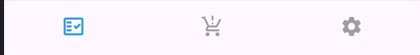
\includegraphics[width=0.3\textwidth]{TFG/img/img/nav.png}

    \caption{Pantalla nav menu (HomeScreen).}
    \label{fig:home_screen}
\end{figure}




     \clearpage

\subsubsection{Pantalla de Gesti\'on de Tareas (\texttt{ToDoScreen})}
\begin{itemize}
    \item \textbf{Descripci\'on}: 
    La pantalla permite gestionar tareas asociadas a un hogar, incluyendo la creaci\'on, edici\'on, eliminaci\'on y marcado de tareas como completadas. Incluye funcionalidades para filtrar tareas y asignarlas a los miembros del hogar.

    \item \textbf{Requisitos}:
    \begin{itemize}
        \item El usuario debe estar autenticado y asociado a un hogar en la base de datos.
        \item Firebase Firestore debe estar configurado correctamente para gestionar la colecci\'on de tareas.
        \item Los miembros del hogar deben estar registrados y visibles en la pantalla.
    \end{itemize}

    \item \textbf{Navegaci\'on}:
    \begin{itemize}
        \item La pantalla muestra una lista de tareas filtradas seg\'un el estado seleccionado: \texttt{Todas}, \texttt{Completadas}, o \texttt{Incompletas}.
        \item Incluye un bot\'on flotante para a\~nadir nuevas tareas y un men\'u emergente para editar tareas existentes.
    \end{itemize}

    \item \textbf{Listado de contenidos}:
    \begin{itemize}
        \item \textbf{Barra superior}:
        \begin{itemize}
            \item Men\'u desplegable para filtrar tareas (\texttt{Todas}, \texttt{Completadas}, \texttt{Incompletas}).
        \end{itemize}
        \item \textbf{Lista de tareas}:
        \begin{itemize}
            \item Muestra tareas con su nombre, categor\'ia y asignaci\'on.
            \item Permite marcar tareas como completadas o incompletas.
            \item Incluye opciones para editar o eliminar tareas.
        \end{itemize}
        \item \textbf{Bot\'on flotante}: 
        \begin{itemize}
            \item Inicia un di\'alogo para a\~nadir una nueva tarea, especificando el nombre, categor\'ia y miembro asignado.
        \end{itemize}
    \end{itemize}

    \item \textbf{Funciones principales}:
    \begin{itemize}
        \item \texttt{\_fetchUserHomeTasks()}:
        \begin{itemize}
            \item Obtiene las tareas asociadas al hogar del usuario desde Firebase Firestore.
        \end{itemize}
        \item \texttt{\_loadTasks()}:
        \begin{itemize}
            \item Carga las tareas del hogar actual y las almacena en la lista de tareas.
        \end{itemize}
        \item \texttt{\_filterTasks()}:
        \begin{itemize}
            \item Aplica filtros a la lista de tareas seg\'un el estado seleccionado.
        \end{itemize}
        \item \texttt{\_addNewTask(String taskName, String category)}:
        \begin{itemize}
            \item A\~nade una nueva tarea a la base de datos y la lista de tareas en la pantalla.
        \end{itemize}
        \item \texttt{\_toggleCompleteTask(int index)}:
        \begin{itemize}
            \item Cambia el estado de una tarea entre completada e incompleta.
        \end{itemize}
        \item \texttt{\_deleteTask(int index)}:
        \begin{itemize}
            \item Elimina una tarea de la base de datos y de la lista en la pantalla.
        \end{itemize}
        \item \texttt{\_editTask(int index, String newTaskName, String newCategory)}:
        \begin{itemize}
            \item Actualiza el nombre y categor\'ia de una tarea existente.
        \end{itemize}
        \item \texttt{\_showAddTaskDialog()}:
        \begin{itemize}
            \item Muestra un di\'alogo para ingresar detalles de una nueva tarea.
        \end{itemize}
        \item \texttt{\_showEditTaskDialog(int index)}:
        \begin{itemize}
            \item Muestra un di\'alogo para editar una tarea seleccionada.
        \end{itemize}
    \end{itemize}
\end{itemize}

\begin{figure}[H]
   
    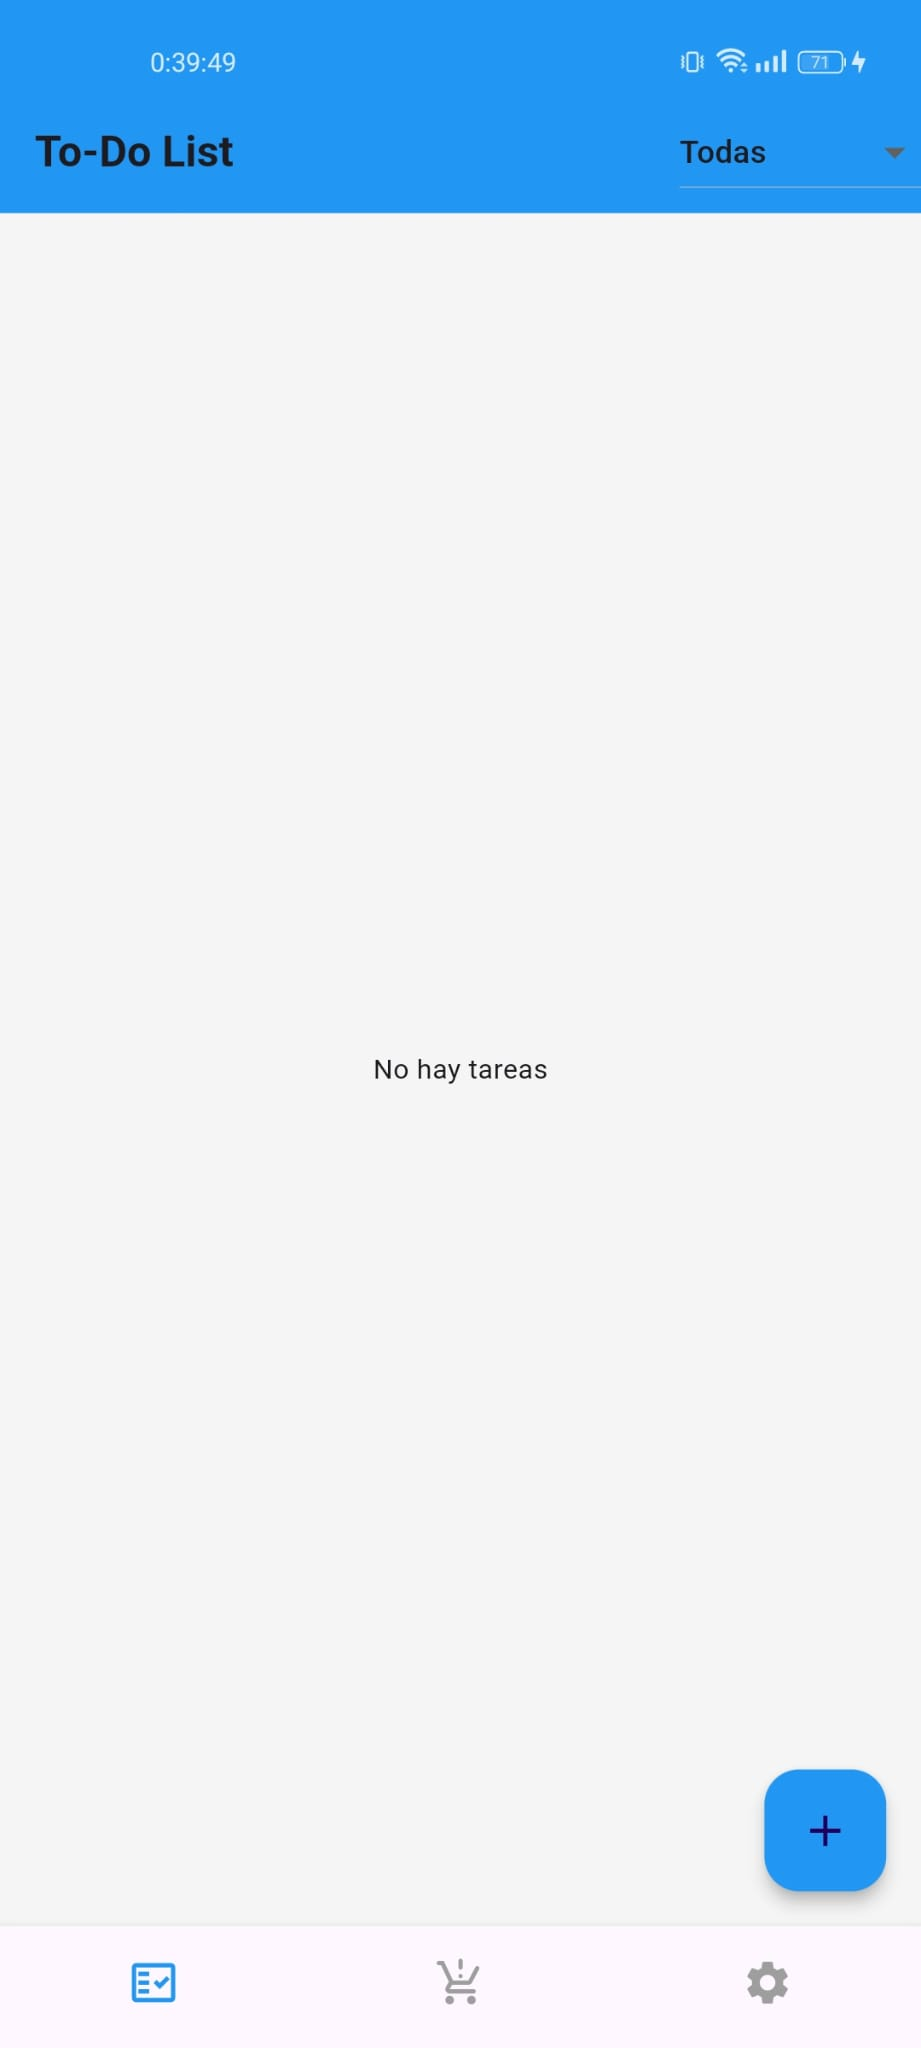
\includegraphics[width=0.3\textwidth]{TFG/img/img/todo.jpeg}
        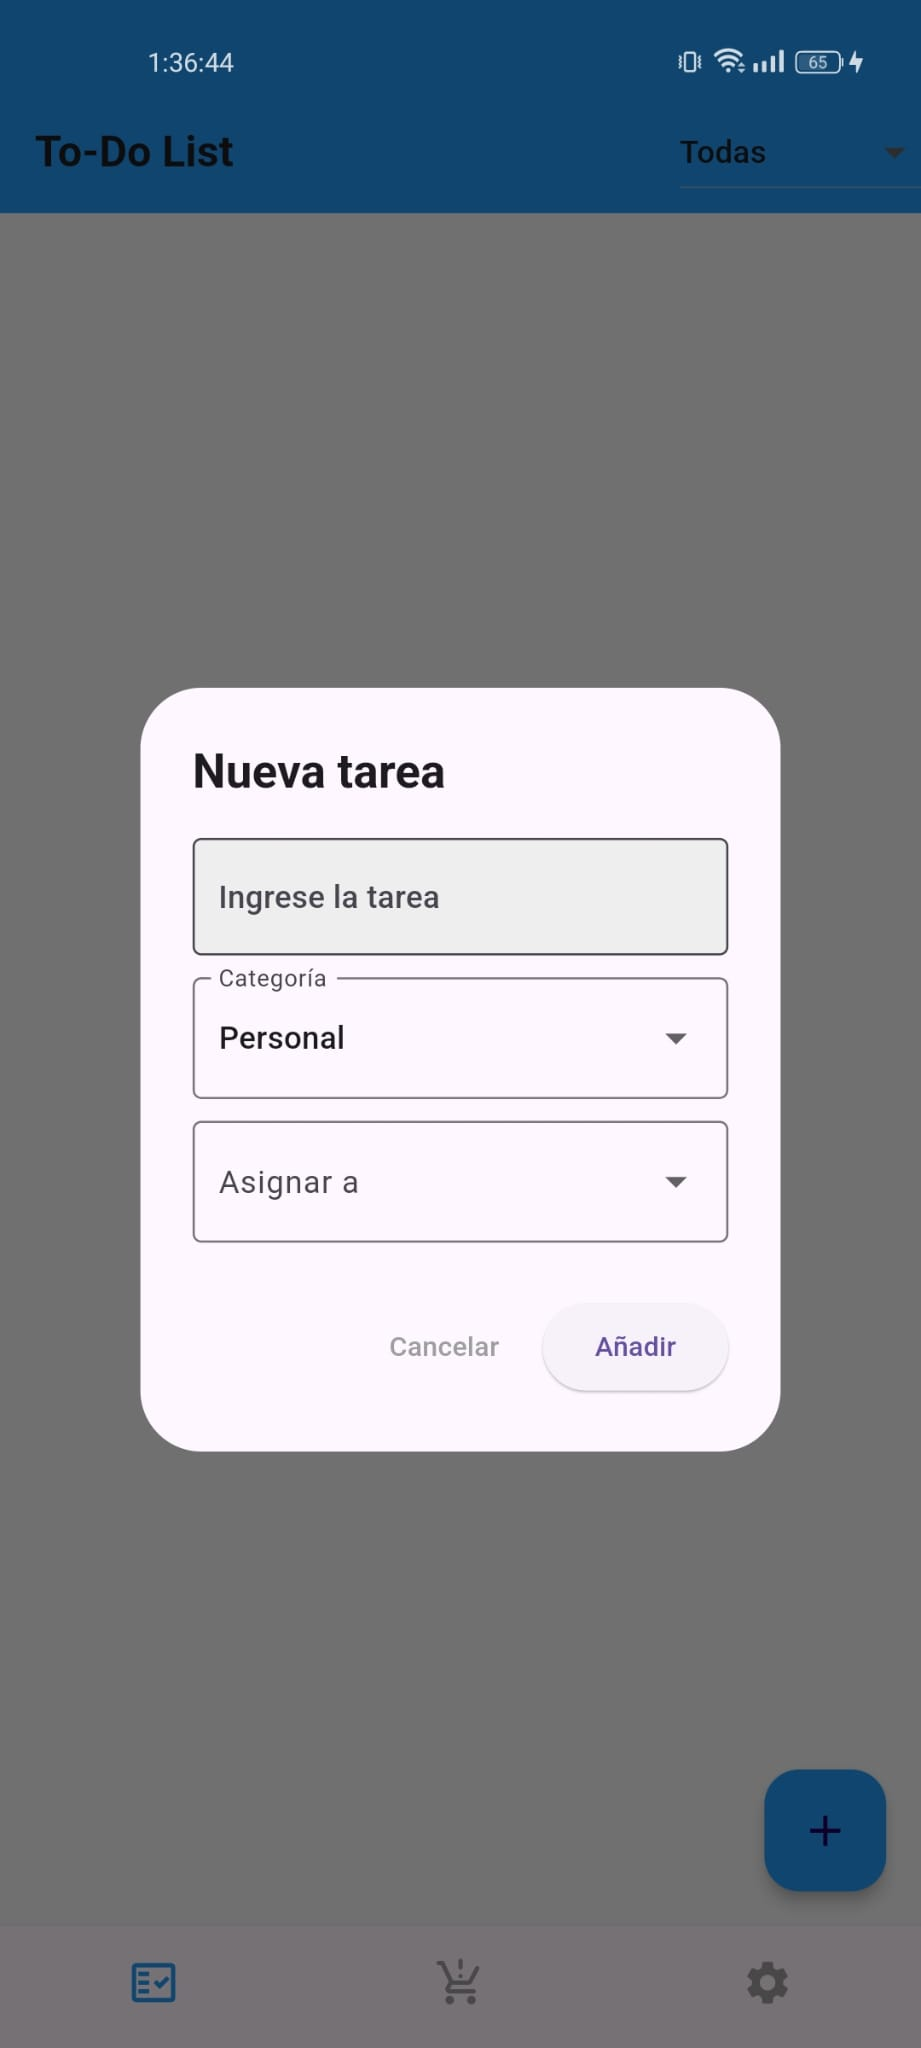
\includegraphics[width=0.3\textwidth]{TFG/img/img/todotarea.jpeg}
   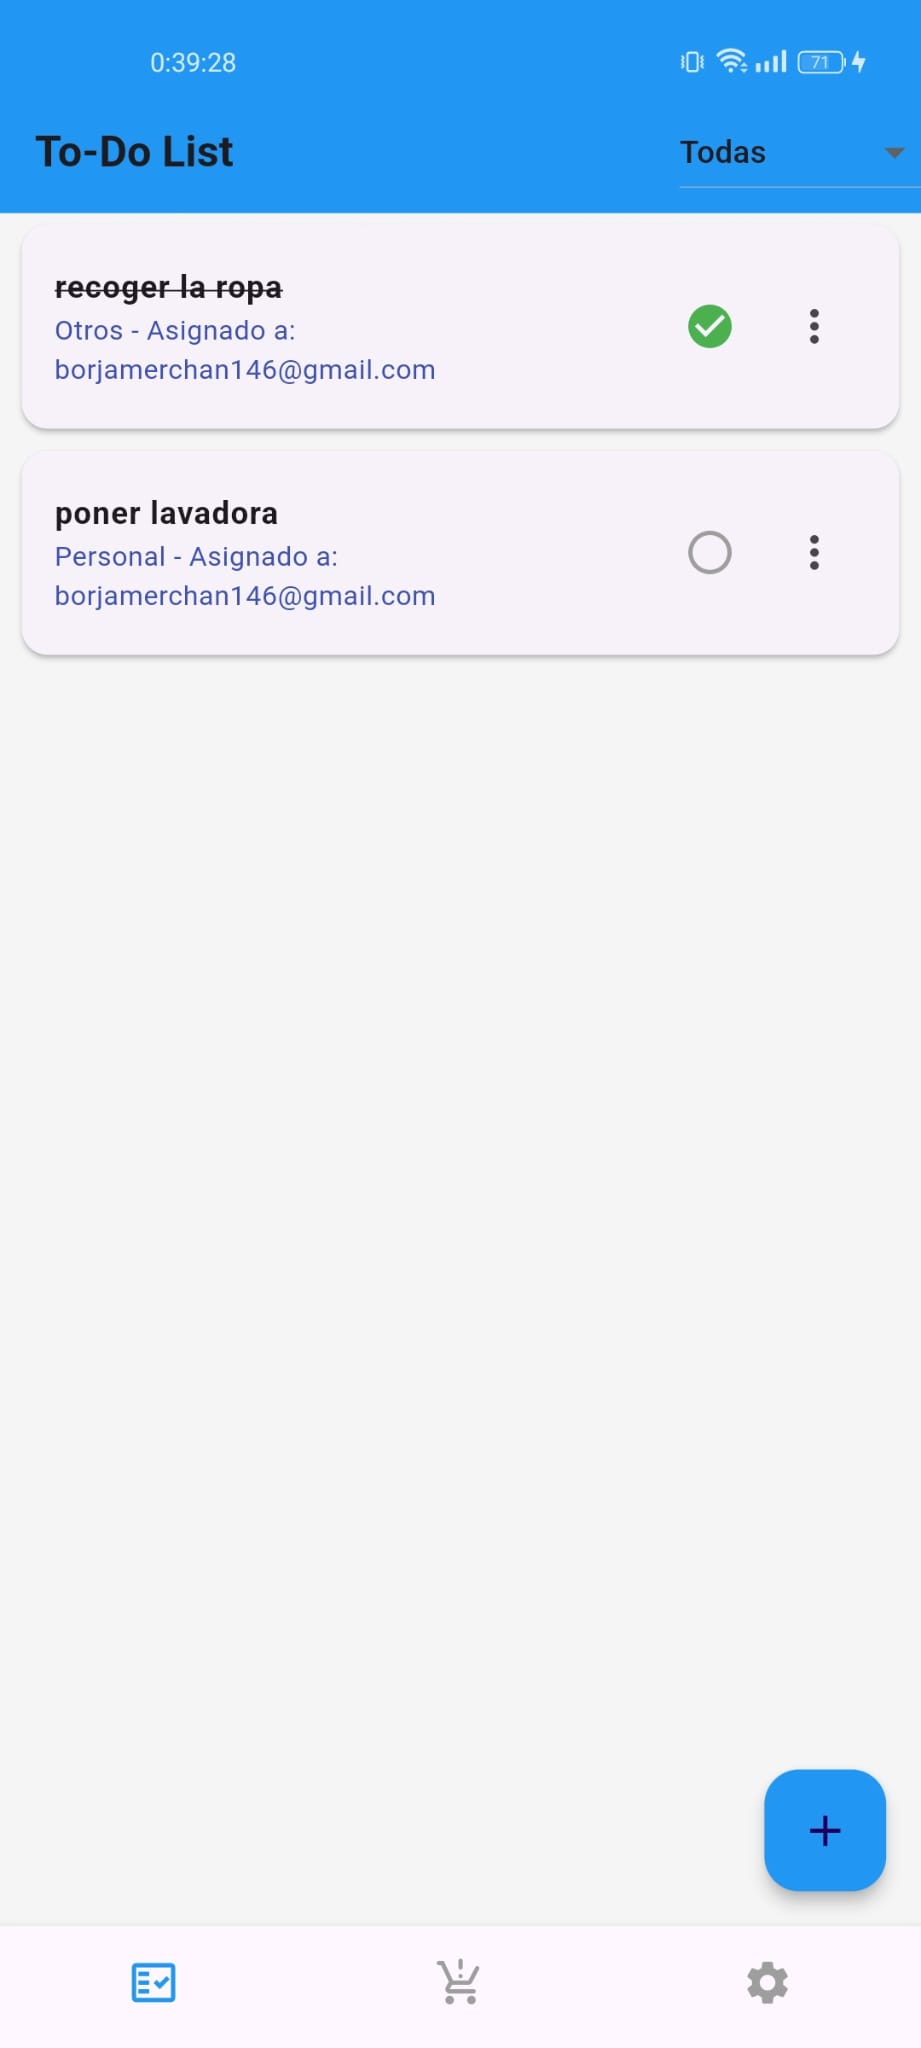
\includegraphics[width=0.3\textwidth]{TFG/img/img/todo1.jpeg}

    \caption{Pantallas de Gesti\'on de Tareas (\texttt{ToDoScreen}).}
    \label{fig:todo_screen}
\end{figure}

\clearpage


\subsubsection{Pantalla de Gesti\'on de Productos (\texttt{NeveraScreen})}
\begin{itemize}
    \item \textbf{Descripci\'on}: 
    Esta pantalla permite gestionar productos asociados a un hogar en un formato de tablero Kanban. Los productos pueden estar en diferentes estados (\texttt{En Nevera} y \texttt{Por Comprar}), ser arrastrados entre columnas, y gestionados mediante opciones como a\~nadir, eliminar o mover productos. Incluye una integraci\'on con la API de Mercadona para explorar categor\'ias y subcategor\'ias de productos.

    \item \textbf{Requisitos}:
    \begin{itemize}
        \item El usuario debe estar autenticado y asociado a un hogar en Firebase Firestore.
        \item Firebase Firestore debe estar configurado correctamente para gestionar los productos.
    \end{itemize}

    \item \textbf{Navegaci\'on}:
    \begin{itemize}
        \item Los productos se organizan en dos columnas principales: \texttt{En Nevera} y \texttt{Por Comprar}.
        \item Los productos pueden ser arrastrados entre columnas para cambiar su estado.
        \item Un bot\'on flotante permite a\~nadir nuevos productos manualmente o desde la API de Mercadona.
        \item Si el usuario realiza un "long click" sobre una tarjeta de producto, este se elimina tanto de la lista visual como de Firebase Firestore.
    \end{itemize}

    \item \textbf{Listado de contenidos}:
    \begin{itemize}
        \item \textbf{Columnas del tablero Kanban}:
        \begin{itemize}
            \item \texttt{En Nevera}: Productos disponibles actualmente en la nevera.
            \item \texttt{Por Comprar}: Productos que a\'un deben adquirirse.
        \end{itemize}
        \item \textbf{Bot\'on flotante}:
        \begin{itemize}
            \item Abre un di\'alogo para a\~nadir productos manualmente o desde la API de Mercadona.
        \end{itemize}
        \item \textbf{Tarjetas de producto}:
        \begin{itemize}
            \item Muestran el nombre, categor\'ia y n\'umero de clics de cada producto.
            \item Incluyen opciones para eliminar productos.
        \end{itemize}
    \end{itemize}

    \item \textbf{Funciones principales}:
    \begin{itemize}
        \item \texttt{\_fetchUserHomeProducts()}:
        \begin{itemize}
            \item Obtiene los productos del hogar del usuario desde Firebase Firestore.
        \end{itemize}
        \item \texttt{\_loadProducts()}:
        \begin{itemize}
            \item Carga los productos en las columnas del tablero Kanban.
            \item Actualiza el contador de clics de cada producto desde Firebase.
        \end{itemize}
        \item \texttt{\_addNewProduct(String productName, String category)}:
        \begin{itemize}
            \item A\~nade un nuevo producto a la base de datos y lo asigna al estado \texttt{Por Comprar}.
        \end{itemize}
        \item \texttt{\_moveProduct(Product product, String newStatus)}:
        \begin{itemize}
            \item Cambia el estado de un producto (\texttt{En Nevera} o \texttt{Por Comprar}) y actualiza la base de datos.
        \end{itemize}
        \item \texttt{\_deleteProduct(String productId)}:
        \begin{itemize}
            \item Elimina un producto de Firebase Firestore y de la lista local.
        \end{itemize}
        \item \texttt{\_handleProductClick(Product product, String status)}:
        \begin{itemize}
            \item Incrementa o decrementa el contador de clics del producto seg\'un su estado.
        \end{itemize}
        \item \texttt{\_showAddProductDialog()}:
        \begin{itemize}
            \item Muestra un di\'alogo para a\~nadir nuevos productos manualmente o desde la API de Mercadona.
        \end{itemize}
        \item \texttt{\_showMercadonaProductsDialog()}:
        \begin{itemize}
            \item Integra la API de Mercadona para explorar categor\'ias y subcategor\'ias de productos.
        \end{itemize}
    \end{itemize}

    \item \textbf{Interacci\'on con la API de Mercadona}:
    \begin{itemize}
        \item Descarga categor\'ias de productos mediante la API de Mercadona.
        \item Permite explorar subcategor\'ias y a\~nadir productos directamente desde la API.
    \end{itemize}
\end{itemize}

\begin{figure}[H]
    
   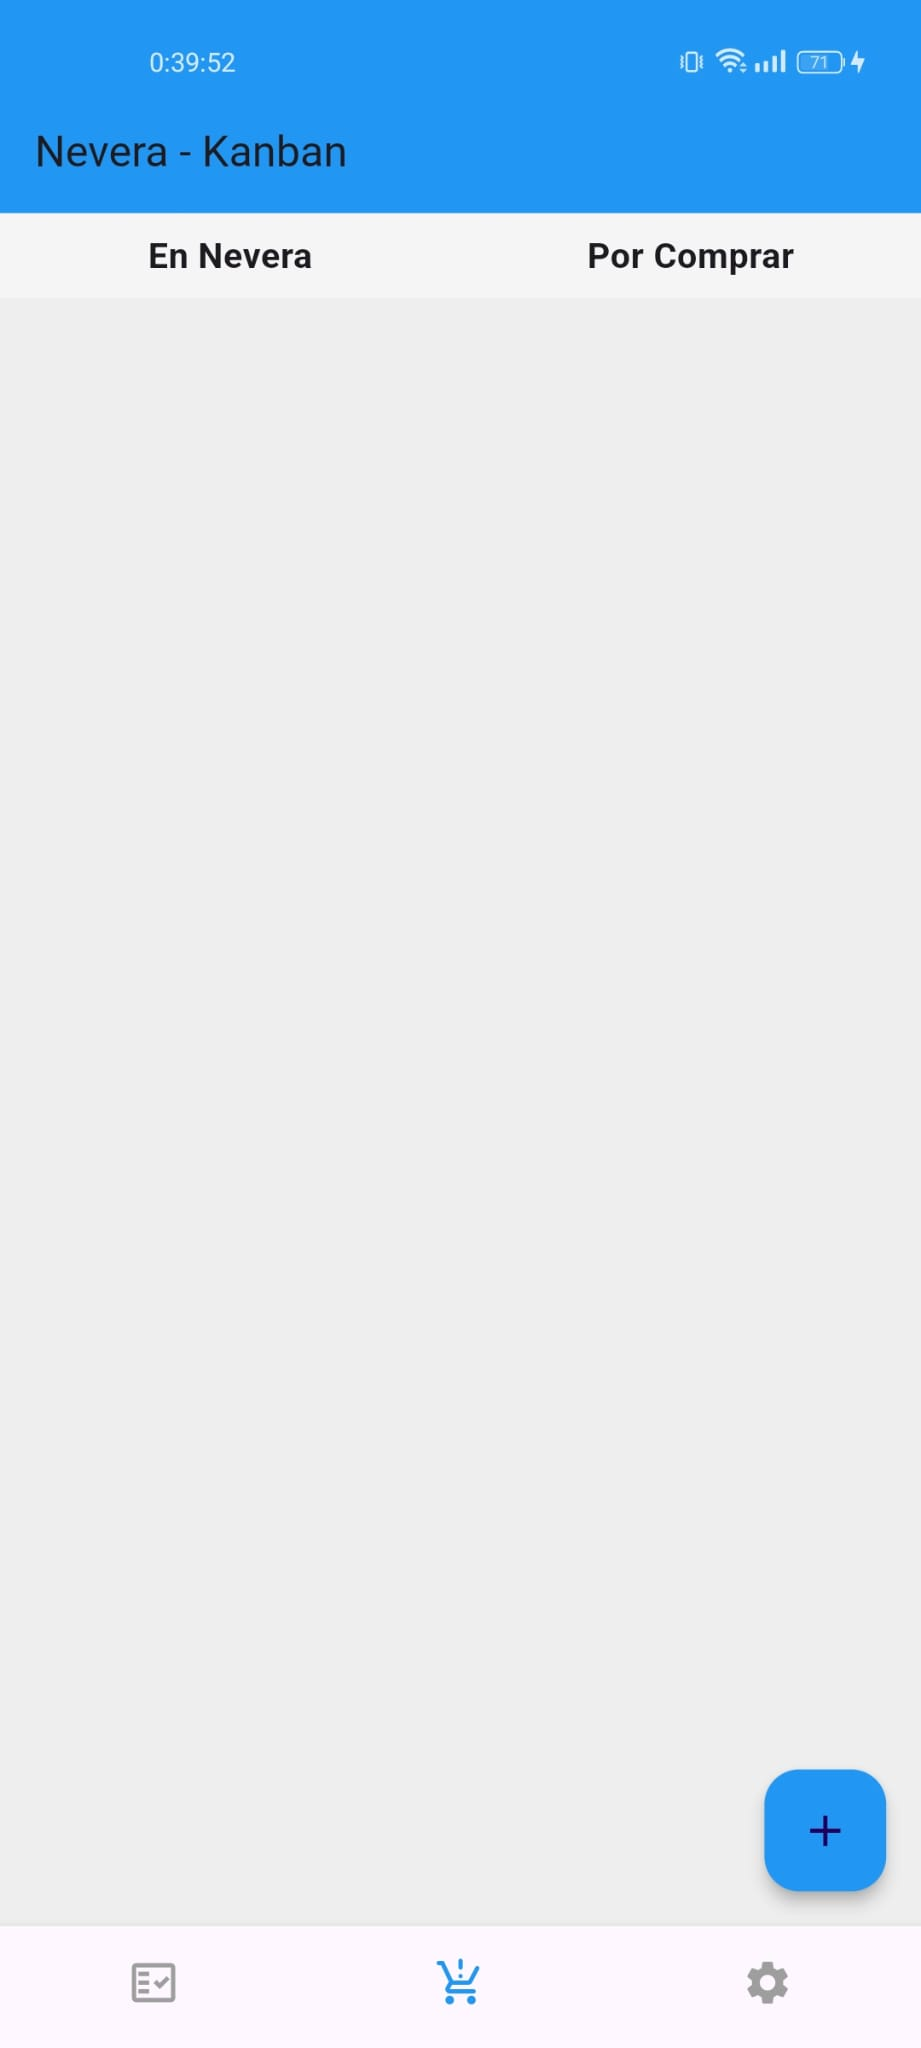
\includegraphics[width=0.3\textwidth]{TFG/img/img/nevera1.jpeg}
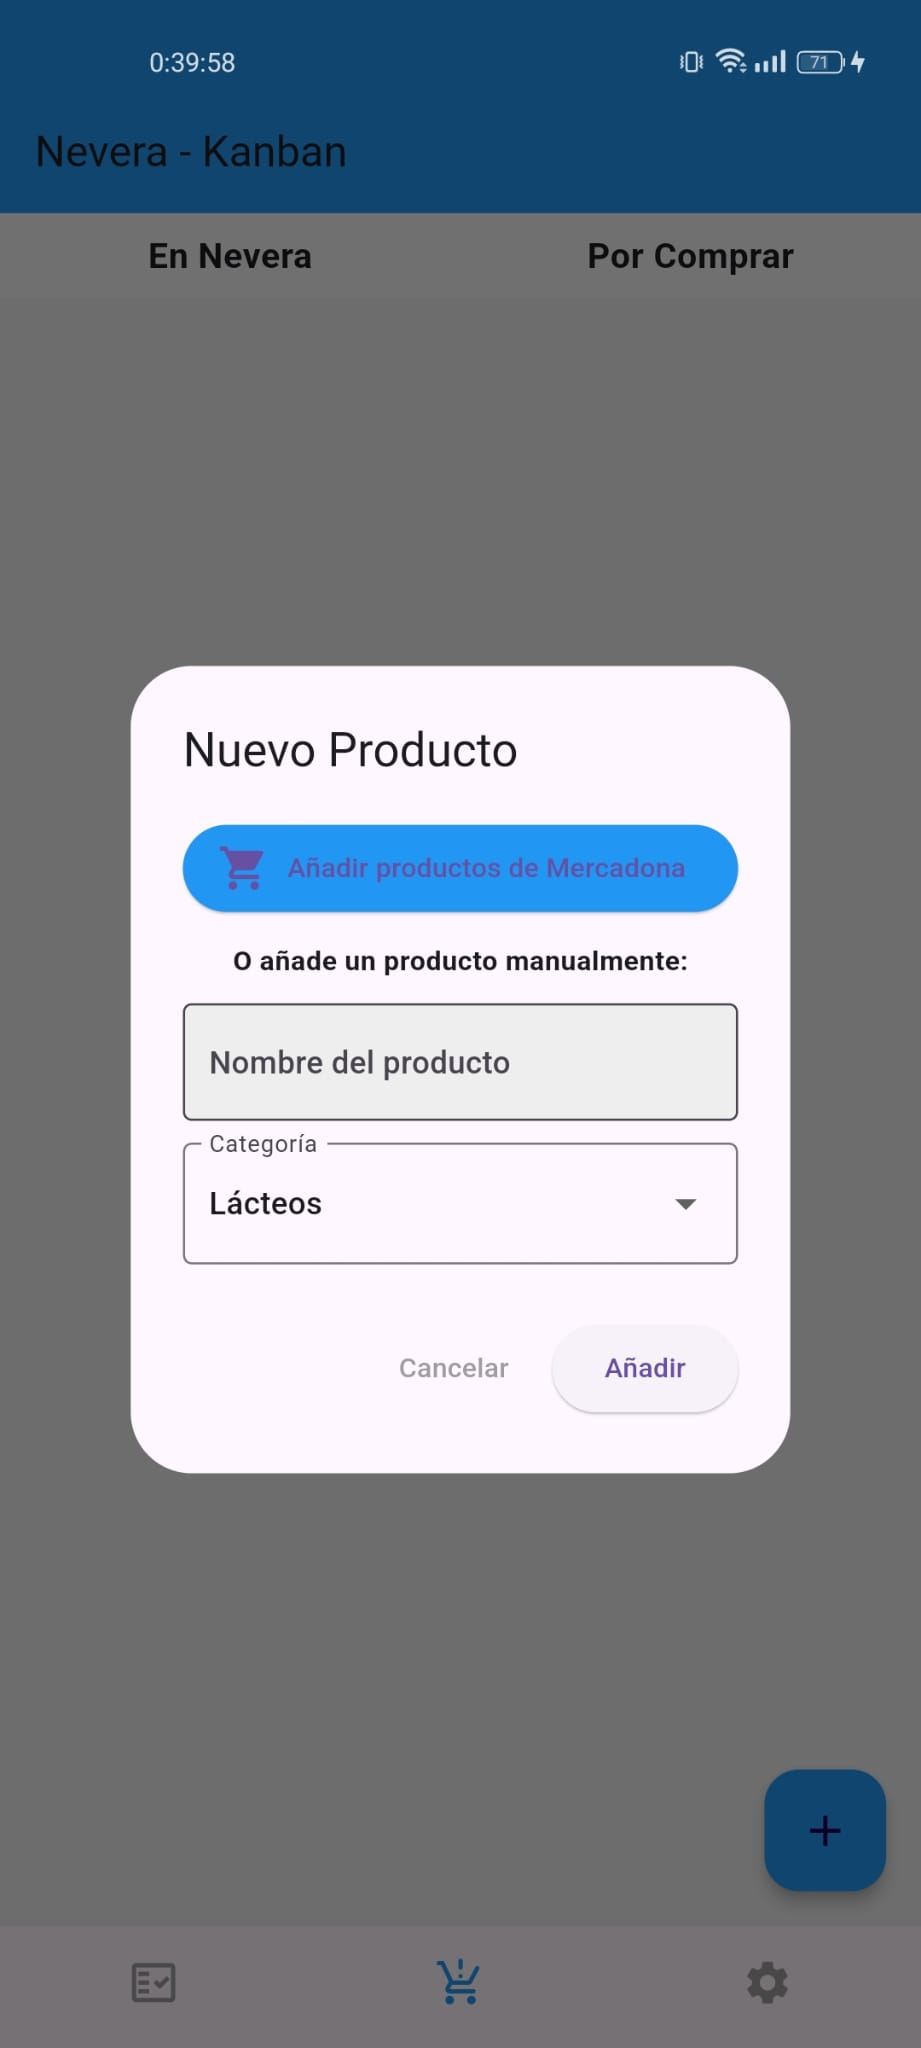
\includegraphics[width=0.3\textwidth]{TFG/img/img/agregar product.jpeg}
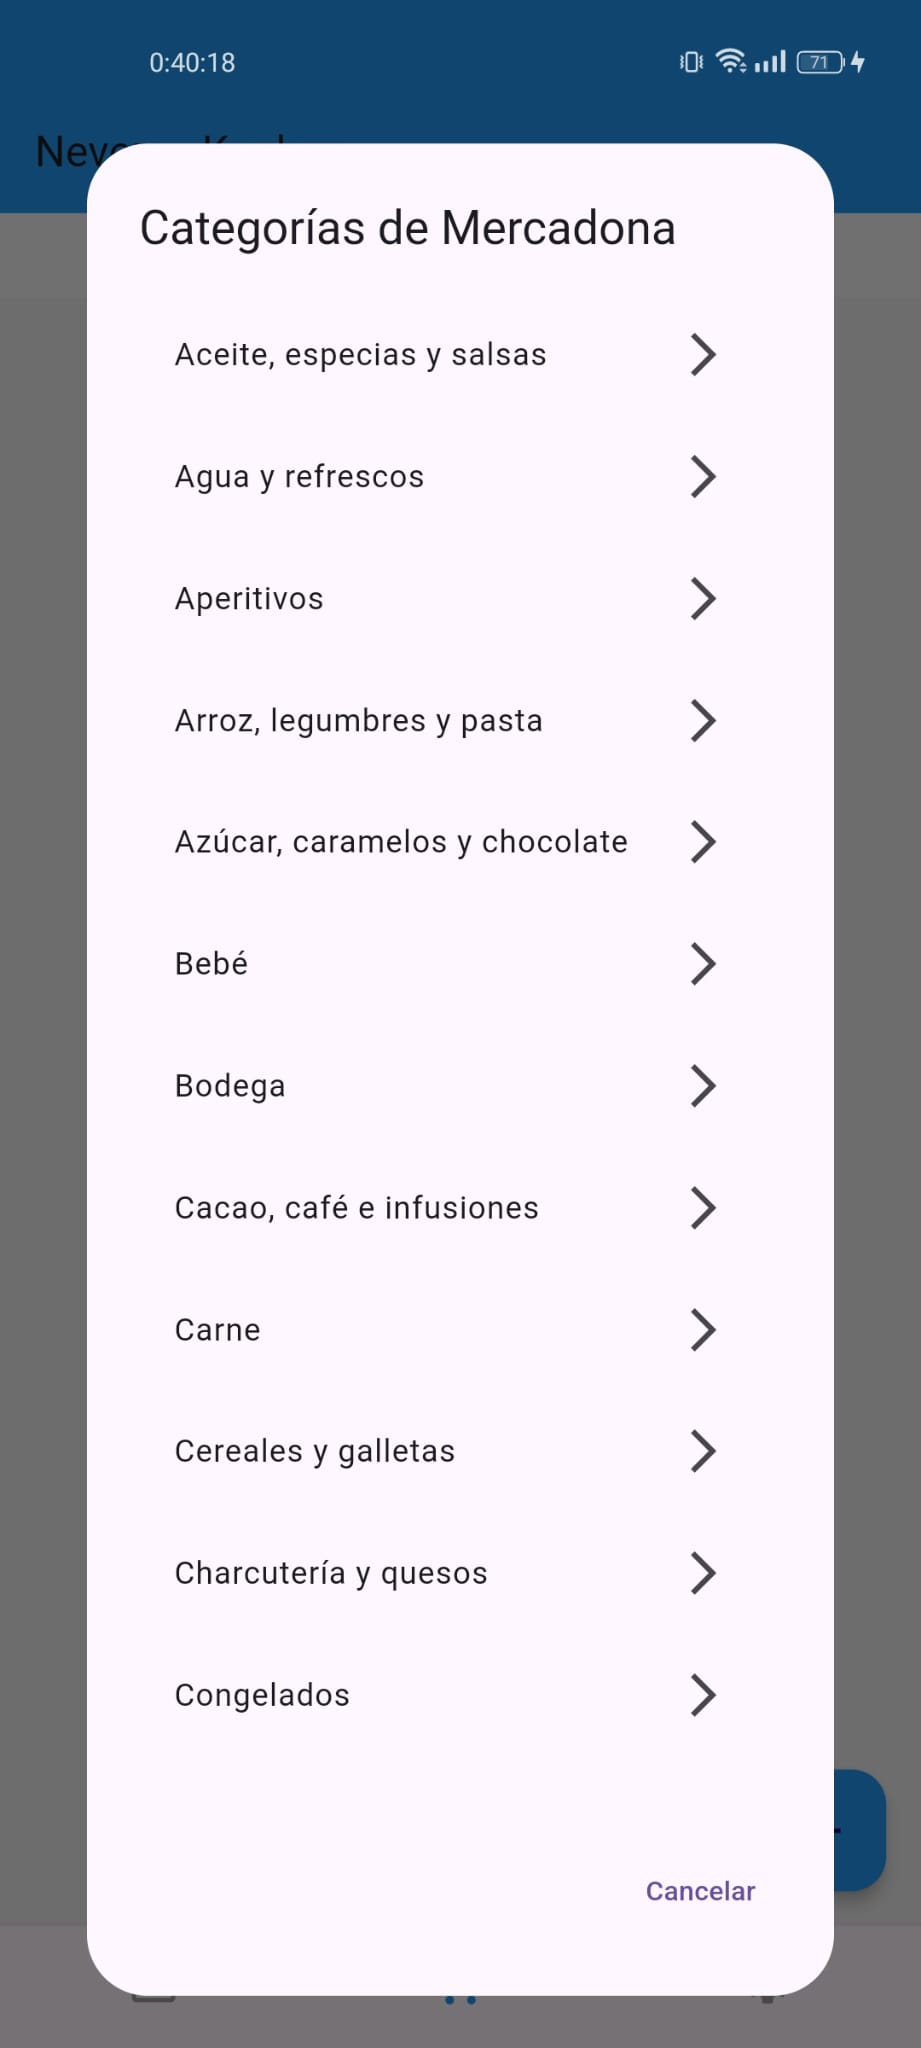
\includegraphics[width=0.3\textwidth]{TFG/img/img/api.jpeg}
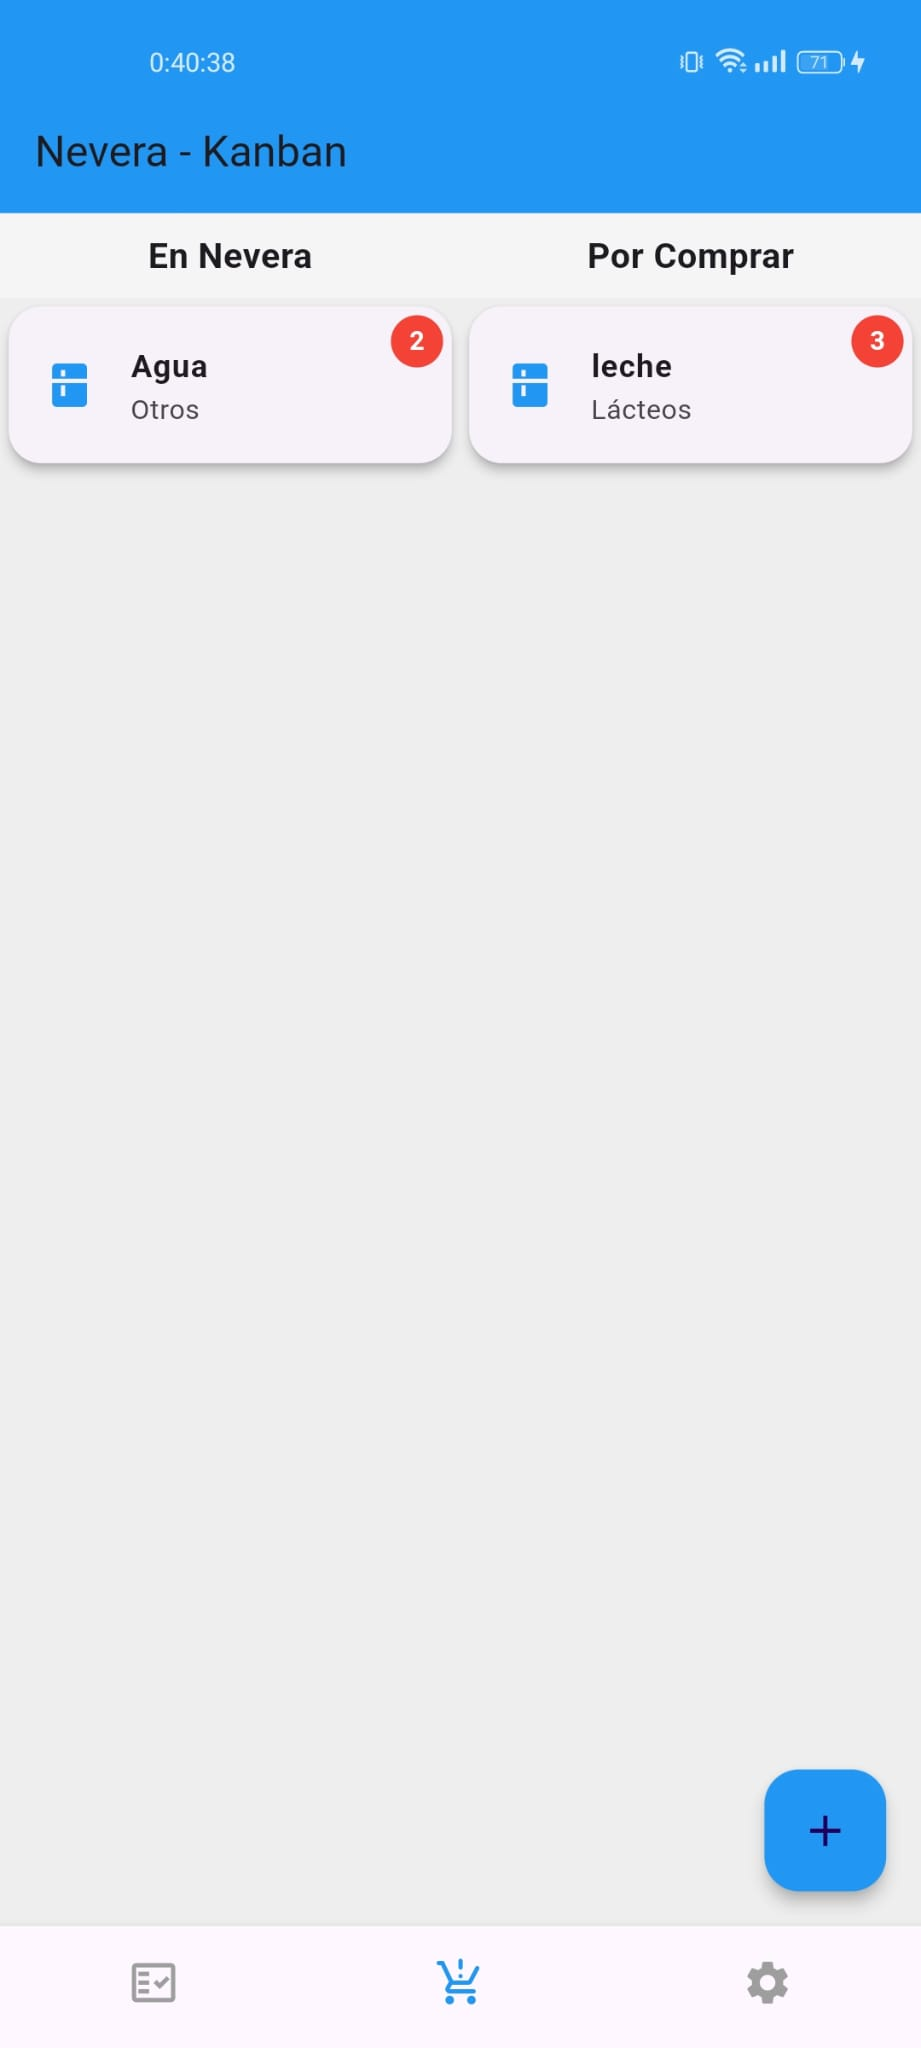
\includegraphics[width=0.3\textwidth]{TFG/img/img/nevera.jpeg}

 
    \caption{Pantallas de Gesti\'on de Productos (\texttt{NeveraScreen}).}
    \label{fig:nevera_screen}
\end{figure}

\clearpage

\subsubsection{Pantalla de Ajustes (\texttt{AjustesScreen})}
\begin{itemize}
    \item \textbf{Descripci\'on}: 
    Esta pantalla permite al usuario visualizar y gestionar ajustes relacionados con su cuenta y hogar. Incluye funcionalidades para seleccionar un grupo de hogar, listar los miembros del hogar y cerrar sesi\'on.

    \item \textbf{Requisitos}:
    \begin{itemize}
        \item El usuario debe estar autenticado en Firebase Authentication.
        \item Firebase Firestore debe estar configurado para almacenar y gestionar los grupos de hogar y sus miembros.
    \end{itemize}

    \item \textbf{Navegaci\'on}:
    \begin{itemize}
        \item El usuario puede visualizar el grupo de hogar que se ha registrado.
        \item Los miembros del hogar seleccionado se muestran en una lista.
        \item Un bot\'on permite cerrar la sesi\'on y redirigir al usuario a la pantalla de inicio de sesi\'on (\texttt{LoginScreen}).
    \end{itemize}

    \item \textbf{Listado de contenidos}:
    \begin{itemize}
        \item \textbf{Avatar del usuario}:
        \begin{itemize}
            \item Muestra una imagen representativa del usuario.
        \end{itemize}
        \item \textbf{Tarjeta de informaci\'on del usuario}:
        \begin{itemize}
            \item Muestra el nombre y correo electr\'onico del usuario autenticado.
        \end{itemize}
        
        \item \textbf{Lista de miembros del hogar}:
        \begin{itemize}
            \item Muestra los correos electr\'onicos de los miembros del hogar seleccionado.
            \item Si no hay miembros disponibles, se muestra un mensaje informativo.
        \end{itemize}
        \item \textbf{Bot\'on de cerrar sesi\'on}:
        \begin{itemize}
            \item Permite al usuario cerrar su sesi\'on y regresar a la pantalla de inicio de sesi\'on.
        \end{itemize}
    \end{itemize}

    \item \textbf{Funciones principales}:
    \begin{itemize}
        \item \texttt{\_fetchUserGroups()}:
        \begin{itemize}
            \item Obtiene los grupos de hogar a los que pertenece el usuario desde Firebase Firestore.
        \end{itemize}
        \item \texttt{\_fetchHomeMembers(String homeName)}:
        \begin{itemize}
            \item Obtiene los miembros del hogar seleccionado desde Firebase Firestore.
        \end{itemize}
        \item \texttt{Cerrar sesi\'on}:
        \begin{itemize}
            \item Cierra la sesi\'on del usuario y redirige a la pantalla de inicio de sesi\'on (\texttt{LoginScreen}).
        \end{itemize}
    \end{itemize}
\end{itemize}

\begin{figure}[H]
    \centering
   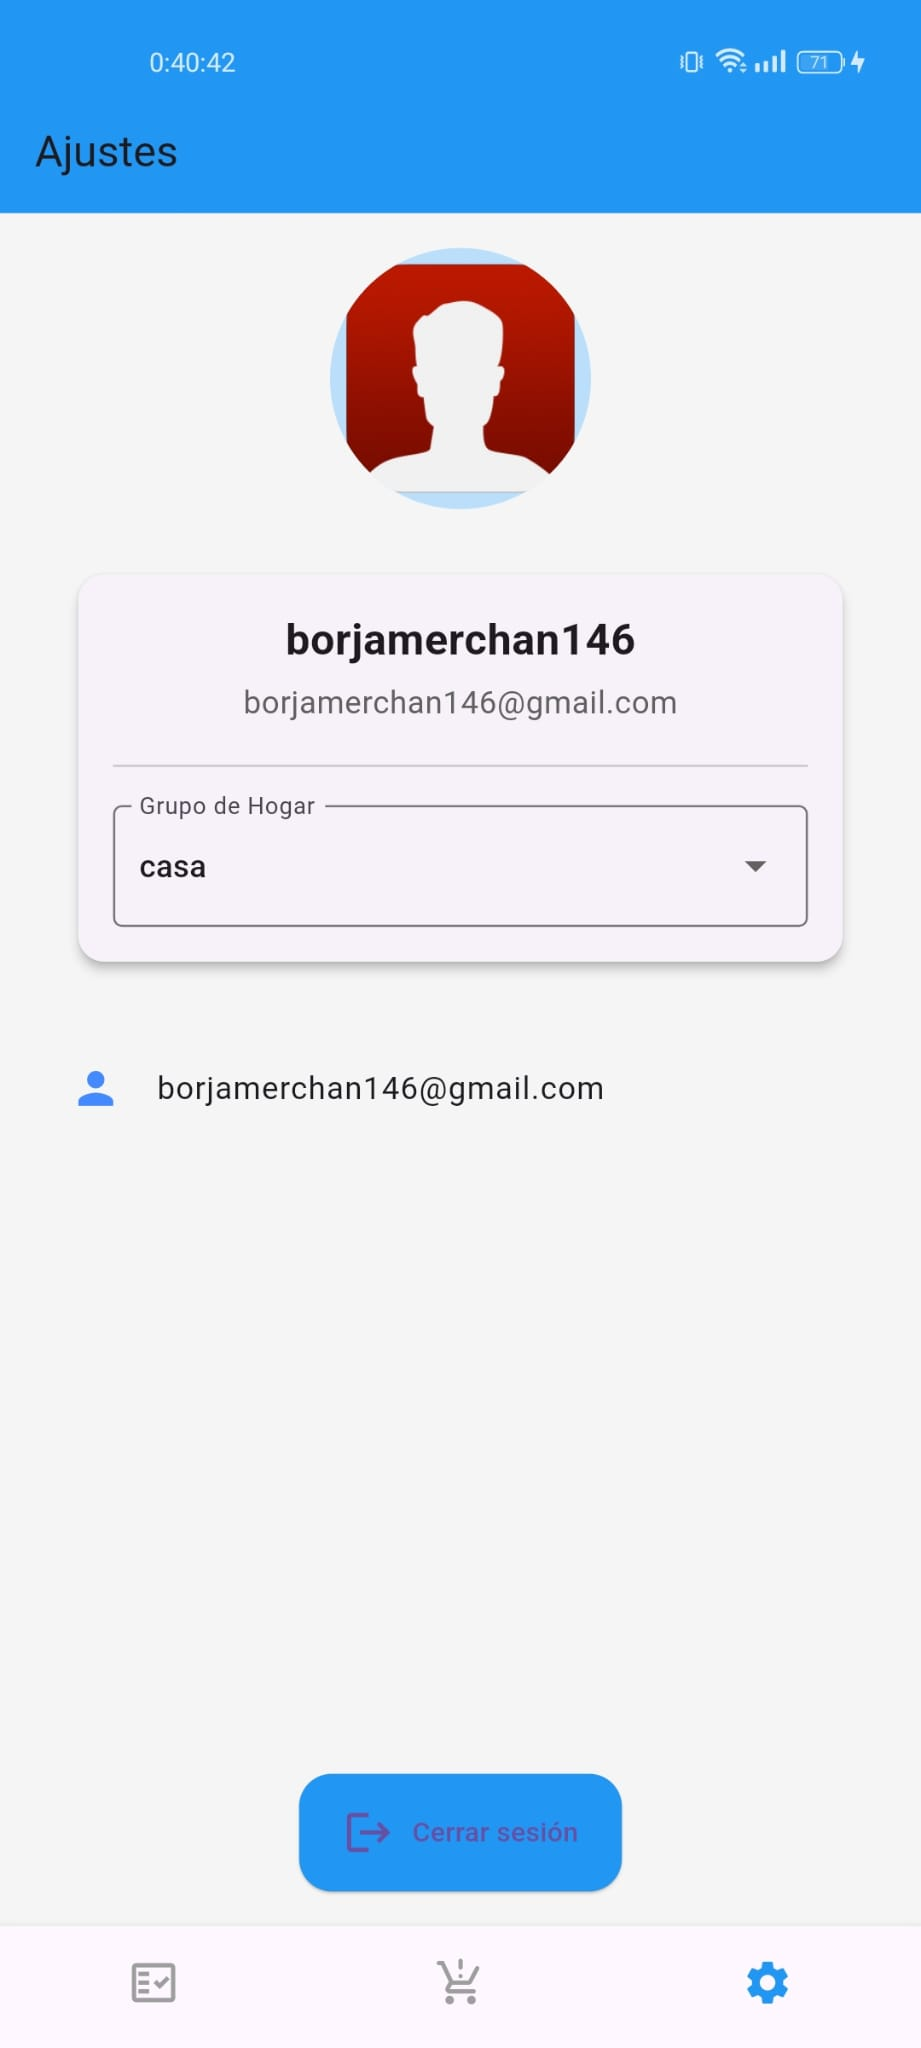
\includegraphics[width=0.3\textwidth]{TFG/img/img/ajustes.jpeg}
    \caption{Pantalla de Ajustes (\texttt{AjustesScreen}).}
    \label{fig:ajustes_screen}
\end{figure}

\clearpage

\section{Biografia}

    \subsection{Documentación}
    \begin{itemize}
        \item \href{https://docs.flutter.dev/get-started/install}{Documentación Offical de flutter}
        \item \href{https://www.apliarte.com/2024/10/implementacion-y-publicacion-de.html}{Información de Como subir la aplicacion ha app store y play store}
        \item \href{https://firebase.google.com/docs/flutter/setup?hl=es&platform=ios}{Documentación Official de firebase }
        \item \href{https://www.youtube.com/watch?v=VOC8gpnGvys}{Importar y exportar datos de firebase}

        \item \href{https://www.youtube.com/watch?v=IOfuM_0Gvvg}{Para exportar usarios de la base de datos de autodentificador}
        \item \href{https://jsoncrack.com/editor}{Tener Dibujado el json en modo visual}

        \item \href{https://www.youtube.com/@HeyFlutter}{Canal de Flutter}

        https://www.youtube.com/@NetNinja
    \end{itemize}

       

    \end{flushleft}
\end{document}

